%%%%%%%%%%%%%%%%%%%%%%%%%%%%%%%%%%%%%%%%%%%%%%%%%%%%%%%%%%%%%%%%%%%%%%%%%%%%%%%%
%% Plantilla de memoria en LaTeX para la EIF - Universidad Rey Juan Carlos
%%
%% Por Gregorio Robles <grex arroba gsyc.urjc.es>
%%     Grupo de Sistemas y Comunicaciones
%%     Escuela de Ingeniería de Fuenlabrada
%%     Universidad Rey Juan Carlos
%% (muchas ideas tomadas de Internet, colegas del GSyC, antiguos alumnos...
%%  etc. Muchas gracias a todos)
%%
%% La última versión de esta plantilla está siempre disponible en:
%%     https://github.com/gregoriorobles/plantilla-memoria
%%
%% Para obtener PDF, ejecuta en la shell:
%%   make
%% (las imágenes deben ir en PNG o JPG)

%%%%%%%%%%%%%%%%%%%%%%%%%%%%%%%%%%%%%%%%%%%%%%%%%%%%%%%%%%%%%%%%%%%%%%%%%%%%%%%%

\documentclass[a4paper, 12pt]{book}
%\usepackage[T1]{fontenc}

\usepackage[a4paper, left=2.5cm, right=2.5cm, top=3cm, bottom=3cm]{geometry}
\usepackage{times}
\usepackage[utf8]{inputenc}
\usepackage[spanish]{babel} % Comenta esta línea si tu memoria es en inglés
\usepackage{url}
\usepackage{color}
%\usepackage[dvipdfm]{graphicx}
\usepackage{graphicx}
\usepackage{subfigure}
\usepackage{float}  %% H para posicionar figuras
\usepackage[nottoc, notlot, notlof, notindex]{tocbibind} %% Opciones de índice
\usepackage{latexsym}  %% Logo LaTeX

\title{Memoria del Proyecto}
\author{Nombre del autor}

\renewcommand{\baselinestretch}{1.5}  %% Interlineado

\begin{document}
	
	\renewcommand{\refname}{Bibliografía}  %% Renombrando
	\renewcommand{\appendixname}{Apéndice}
	
	
	%%%%%%%%%%%%%%%%%%%%%%%%%%%%%%%%%%%%%%%%%%%%%%%%%%%%%%%%%%%%%%%%%%%%%%%%%%%%%%%%
	% PORTADA
	
	\begin{titlepage}
		\begin{center}
			\includegraphics[scale=0.6]{img/URJ_logo_Color_POS.png}
			
			\vspace{1.75cm}
			
			\LARGE
			ESCUELA DE INGENIERÍA DE FUENLABRADA
			\vspace{1cm}
			
			\LARGE
			GRADO EN INGENIERÍA EN TECNOLOGÍAS DE LA TELECOMUNICACIÓN
			
			\vspace{1cm}
			\LARGE
			\textbf{TRABAJO FIN DE GRADO}
			
			\vspace{1cm}
			
			\Large
			CONFIGURACIÓN Y PRUEBAS DE UN PLANO DE CONTROL IN-BAND SDN/OPENFLOW: MAQUETA CON SWITCHES ETHERNET  
			
			\vspace{2cm}
			
			\large
			Autor : Luis Haro Peña \\
			Tutor : Pedro de las Heras Quirós\\
			Cotutor: Eva María Castro Barbero
			\vspace{1cm}
			
			\large
			Curso académico 2023/2024
			
		\end{center}
	\end{titlepage}
	
	\newpage
	\mbox{}
	\thispagestyle{empty} % para que no se numere esta pagina
	
	
	
	%%%%%%%%%%%%%%%%%%%%%%%%%%%%%%%%%%%%%%%%%%%%%%%%%%%%%%%%%%%%%%%%%%%%%%%%%%%%%%%%
	%%%% Para firmar
	\clearpage
	\pagenumbering{gobble}
	\chapter*{}
	
	\vspace{-4cm}
	\begin{center}
		\LARGE
		\textbf{Trabajo Fin de Grado}
		
		\vspace{1cm}
		\large
		Configuración y Pruebas de un Plano de Control In-Band SDN/Openflow: Maqueta con Switches Ethernet
		
		\vspace{1cm}
		\large
		\textbf{Autor :} Luis Haro Peña \\
		\textbf{Tutor :} Pedro de las Heras Quirós
		
	\end{center}
	
	\vspace{1cm}
	La defensa del presente Proyecto Fin de Carrera se realizó el día \qquad$\;\,$ de \qquad\qquad\qquad\qquad \newline de 2023, siendo calificada por el siguiente tribunal:
	
	
	\vspace{0.5cm}
	\textbf{Presidente:}
	
	\vspace{1.2cm}
	\textbf{Secretario:}
	
	\vspace{1.2cm}
	\textbf{Vocal:}
	
	
	\vspace{1.2cm}
	y habiendo obtenido la siguiente calificación:
	
	\vspace{1cm}
	\textbf{Calificación:}
	
	
	\vspace{1cm}
	\begin{flushright}
		Fuenlabrada, a \qquad$\;\,$ de \qquad\qquad\qquad\qquad de 2024
	\end{flushright}
	
	
	%%%%%%%%%%%%%%%%%%%%%%%%%%%%%%%%%%%%%%%%%%%%%%%%%%%%%%%%%%%%%%%%%%%%%%%%%%%%%%%%
	%%%% Agradecimientos
	
	\chapter*{Agradecimientos}
	%\addcontentsline{toc}{chapter}{Agradecimientos} % si queremos que aparezca en el índice
	\markboth{AGRADECIMIENTOS}{AGRADECIMIENTOS} % encabezado 
	
	Estimada familia, pareja, amigos y seres queridos,
	
	Hoy quiero tomar un momento para expresar mi más profundo agradecimiento por todo su apoyo y amor incondicional durante mi trayectoria académica y, en particular, en la culminación de mi TFG. Vuestra presencia constante, apoyo y comprensión han sido fundamentales en mi camino hacia el éxito.
	
	
	Con gratitud,
	Luis.
	
	%%%%%%%%%%%%%%%%%%%%%%%%%%%%%%%%%%%%%%%%%%%%%%%%%%%%%%%%%%%%%%%%%%%%%%%%%%%%%%%%
	%%%% Resumen
	
	\chapter*{Resumen}
	%\addcontentsline{toc}{chapter}{Resumen} % si queremos que aparezca en el índice
	\markboth{RESUMEN}{RESUMEN} % encabezado
	
	Este Trabajo de Fin de Grado se centra en el diseño, configuración y pruebas de un plano de control in-band basado en SDN/Openflow para una maqueta con switches Ethernet. La creciente demanda de redes más flexibles, escalables y programables ha impulsado el desarrollo de nuevas tecnologías como la Red Definida por Software (SDN) y el protocolo Openflow. En este contexto, se busca implementar un plano de control in-band utilizando estos conceptos para habilitar la gestión y control centralizado de la red.
	
	El objetivo principal de este estudio es establecer una infraestructura de red SDN/Openflow utilizando switches Ethernet y evaluar su rendimiento y funcionalidad a través de pruebas exhaustivas. Se llevará a cabo la configuración de los switches y su conexión con el controlador SDN para lograr la comunicación entre ambos. Se implementarán políticas de enrutamiento y se realizarán pruebas de rendimiento y escalabilidad para evaluar la eficiencia de la solución propuesta. Los resultados obtenidos permitirán analizar el impacto de la configuración y los ajustes en la calidad del servicio y en la capacidad de gestión de la red, proporcionando una base sólida para futuras implementaciones de redes SDN/Openflow en entornos de telecomunicaciones.
	
	Además, se abordará la cuestión de la seguridad en el entorno SDN/Openflow, ya que la gestión centralizada introduce nuevos desafíos en cuanto a la protección de la red contra amenazas cibernéticas. Se realizará un análisis exhaustivo de las vulnerabilidades potenciales y se propondrán medidas de seguridad para mitigar los riesgos asociados. Esto incluirá la implementación de políticas de acceso y autenticación, el monitoreo constante de la red y la aplicación de mecanismos de detección y respuesta ante intrusiones.
	
	En resumen, este trabajo de fin de grado se enfoca en la configuración y pruebas de un plano de control in-band SDN/Openflow en una maqueta con switches Ethernet. Se pretende demostrar la viabilidad de esta solución para la gestión centralizada de redes, evaluando su rendimiento, escalabilidad y seguridad. Los resultados y conclusiones obtenidos serán de gran valor para futuros proyectos en el ámbito de las telecomunicaciones, contribuyendo al avance y desarrollo de las redes definidas por software y el paradigma SDN/Openflow.
	
	%%%%%%%%%%%%%%%%%%%%%%%%%%%%%%%%%%%%%%%%%%%%%%%%%%%%%%%%%%%%%%%%%%%%%%%%%%%%%%%%
	%%%% Resumen en inglés
	
	\chapter*{Summary}
	%\addcontentsline{toc}{chapter}{Summary} % si queremos que aparezca en el índice
	\markboth{SUMMARY}{SUMMARY} % encabezado
	
	This Final Degree Project focuses on the design, configuration and testing of an SDN/Openflow based in-band control plane for an Ethernet switch layout. The growing demand for more flexible, scalable and programmable networks has driven the development of new technologies such as Software Defined Networking (SDN) and the Openflow protocol. In this context, we seek to implement an in-band control plane using these concepts to enable centralized network management and control.
	
	The main objective of this study is to establish an SDN/Openflow network infrastructure using Ethernet switches and evaluate its performance and functionality through extensive testing. The configuration of the switches and their connection to the SDN controller will be carried out to achieve communication between the two. Routing policies will be implemented and performance and scalability tests will be performed to evaluate the efficiency of the proposed solution. The results obtained will allow analyzing the impact of the configuration and adjustments on the quality of service and network manageability, providing a solid basis for future implementations of SDN/Openflow networks in telecommunication environments.
	
	In addition, the issue of security in the SDN/Openflow environment will be addressed, as centralized management introduces new challenges in terms of protecting the network against cyber threats. A comprehensive analysis will be conducted
	
	
	%%%%%%%%%%%%%%%%%%%%%%%%%%%%%%%%%%%%%%%%%%%%%%%%%%%%%%%%%%%%%%%%%%%%%%%%%%%%%%%%
	%%%%%%%%%%%%%%%%%%%%%%%%%%%%%%%%%%%%%%%%%%%%%%%%%%%%%%%%%%%%%%%%%%%%%%%%%%%%%%%%
	% ÍNDICES %
	%%%%%%%%%%%%%%%%%%%%%%%%%%%%%%%%%%%%%%%%%%%%%%%%%%%%%%%%%%%%%%%%%%%%%%%%%%%%%%%%
	
	% Las buenas noticias es que los índices se generan automáticamente.
	% Lo único que tienes que hacer es elegir cuáles quieren que se generen,
	% y comentar/descomentar esa instrucción de LaTeX.
	
	%%%% Índice de contenidos
	\tableofcontents 
	%%%% Índice de figuras
	\cleardoublepage
	%\addcontentsline{toc}{chapter}{Lista de figuras} % para que aparezca en el indice de contenidos
	\listoffigures % indice de figuras
	%%%% Índice de tablas
	%\cleardoublepage
	%\addcontentsline{toc}{chapter}{Lista de tablas} % para que aparezca en el indice de contenidos
	%\listoftables % indice de tablas
	
	
	%%%%%%%%%%%%%%%%%%%%%%%%%%%%%%%%%%%%%%%%%%%%%%%%%%%%%%%%%%%%%%%%%%%%%%%%%%%%%%%%
	%%%%%%%%%%%%%%%%%%%%%%%%%%%%%%%%%%%%%%%%%%%%%%%%%%%%%%%%%%%%%%%%%%%%%%%%%%%%%%%%
	% INTRODUCCIÓN %
	%%%%%%%%%%%%%%%%%%%%%%%%%%%%%%%%%%%%%%%%%%%%%%%%%%%%%%%%%%%%%%%%%%%%%%%%%%%%%%%%
	
	\clearpage
	\chapter{Introducción}
	\label{sec:intro} % etiqueta para poder referenciar luego en el texto con ~\ref{sec:intro}
	\pagenumbering{arabic} % para empezar la numeración de página con números
	
	
	En el ámbito de las telecomunicaciones, la evolución constante de las redes y la creciente demanda de mayor flexibilidad y eficiencia han impulsado el surgimiento de nuevas tecnologías y enfoques de gestión de redes. Entre ellos, destaca la Red Definida por Software (SDN) y el protocolo Openflow, los cuales han revolucionado la forma en que se configuran y controlan las redes. En este contexto, el presente Trabajo de Fin de Grado se enfoca en la Configuración y Pruebas de un Plano de Control In-Band SDN/Openflow, específicamente en una maqueta con switches Ethernet.
	
	El objetivo principal de este trabajo es explorar las capacidades y ventajas que ofrece la implementación de un plano de control in-band SDN/Openflow en una infraestructura de red basada en switches Ethernet. A través de la configuración y pruebas exhaustivas, se busca demostrar la viabilidad y el potencial de esta solución en términos de gestión centralizada, flexibilidad y escalabilidad. Además, se abordará el aspecto de la seguridad, ya que la introducción de un plano de control centralizado también conlleva desafíos en cuanto a la protección contra amenazas cibernéticas.
	
	Este trabajo se estructura en diferentes fases, comenzando por una revisión exhaustiva de la literatura y los conceptos fundamentales relacionados con SDN, Openflow y la configuración de redes Ethernet. A continuación, se procederá a la implementación del plano de control in-band, incluyendo la configuración de los switches y su interconexión con el controlador SDN. Posteriormente, se llevarán a cabo pruebas de rendimiento y escalabilidad para evaluar el desempeño de la solución propuesta. Además, se analizará la seguridad de la red implementada y se propondrán medidas de protección.
	
	Los resultados y conclusiones de este trabajo serán de gran relevancia para el campo de las telecomunicaciones, ya que proporcionarán información valiosa sobre la efectividad y el impacto de la configuración y pruebas de un plano de control in-band SDN/Openflow en una infraestructura de switches Ethernet. Además, se contribuirá al conocimiento existente en términos de seguridad en entornos SDN, brindando recomendaciones prácticas para mitigar posibles vulnerabilidades. En última instancia, se espera que este estudio sirva como base para futuras implementaciones de redes SDN/Openflow, impulsando la evolución y la eficiencia en la gestión de redes de telecomunicaciones.
	
	\section{Contexto}
	\label{chap:estado}
	Dicho esto, utilizaremos este apartado del trabajo para definir los conceptos que se van a tratar a lo largo de la investigación:
	- Switch. También conocido como "conmutador en red",un dispositivo físico que funciona en la capa de enlace de datos (Data Link) del modelo de interconexión de sistemas abiertos (OSI) o la Capa 2. Recibe los paquetes enviados por los dispositivos conectados a sus puertos físicos y los reenvía a los dispositivos a los que están destinados los paquetes. Los conmutadores también pueden operar en la capa de red (Capa 3), donde se produce el enrutamiento.
	
	Los conmutadores son un componente habitual de las redes basadas en ethernet, fibra, Modo de Transferencia Asíncrona (ATM) e InfiniBand, entre otras. Sin embargo, la mayoría de los conmutadores actuales utilizan ethernet. Una vez que un dispositivo se conecta a un conmutador, éste anota su dirección de control de acceso al medio (MAC), un código que está incorporado en la tarjeta de interfaz de red (NIC) del dispositivo. El conmutador utiliza la dirección MAC para identificar qué paquetes salientes del dispositivo se envían y dónde entregar los paquetes entrantes.
	
	La dirección MAC identifica el dispositivo físico y no cambia, mientras que la dirección IP de la capa de red (Capa 3), puede ser asignada dinámicamente a un dispositivo y cambiar con el tiempo. (Piensa en la dirección MAC como el número de bastidor de un coche y en la dirección IP como la matrícula).
	
	Cuando un paquete entra en el conmutador, éste lee su cabecera, luego compara la dirección o direcciones de destino y envía el paquete a través de los puertos apropiados que conducen a los dispositivos de destino.
	
	Para reducir la posibilidad de colisiones entre el tráfico de red que entra y sale de un conmutador y un dispositivo conectado al mismo tiempo, la mayoría de los conmutadores ofrecen una funcionalidad full-duplex en la que los paquetes que entran y salen de un dispositivo tienen acceso a todo el ancho de banda de la conexión del conmutador. (Imagínate a dos personas hablando por un smartphone en lugar de por un walkie-talkie).
	
	Si bien es cierto que los conmutadores funcionan en la Capa 2, también pueden funcionar en la Capa 3, lo que es necesario para que admitan las LAN virtuales (VLAN), segmentos de red lógicos que pueden abarcar subredes. Para que el tráfico vaya de una subred a otra debe pasar entre conmutadores, lo que se facilita con las capacidades de enrutamiento integradas en los conmutadores. 
	
	En pocas palabras, se trata de un dispositivo que sirve para conectar varios elementos dentro de una red.
	
	\section{Redes de Ordenadores} 
	\label{sec:redes}
	
	Las redes de ordenadores son sistemas interconectados que permiten la comunicación y el intercambio de datos entre diferentes dispositivos informáticos. Estas redes pueden ser locales (LAN), que conectan dispositivos en un área geográfica limitada, o extenderse a través de distancias más grandes, como en las redes de área amplia (WAN) o incluso redes globales como Internet.
	
	En una red de ordenadores, los dispositivos, como computadoras, servidores, impresoras y dispositivos de almacenamiento, se conectan mediante cables o tecnologías inalámbricas. La comunicación se facilita a través de protocolos y estándares, como TCP/IP (Protocolo de Control de Transmisión/Protocolo de Internet).
	
	Las redes pueden clasificarse según su topología (la disposición física de los componentes), su tamaño y su uso específico. Las tecnologías asociadas incluyen Ethernet, Wi-Fi, VPN (Red Privada Virtual), y dispositivos como routers y switches que gestionan el flujo de datos en la red. Las redes de ordenadores son fundamentales en la actualidad para la comunicación, el acceso a recursos compartidos y la colaboración en entornos empresariales y domésticos.
	
	%%%%%%%%%%%%%%%%%%%%%%%%%%%%%%%%%%%%%%%%%%%%%%%%%%%%%%%%%%%%%%%%%%%%%%%%%%%%%%%%
	%%%%%%%%%%%%%%%%%%%%%%%%%%%%%%%%%%%%%%%%%%%%%%%%%%%%%%%%%%%%%%%%%%%%%%%%%%%%%%%%
	% OBJETIVOS %
	%%%%%%%%%%%%%%%%%%%%%%%%%%%%%%%%%%%%%%%%%%%%%%%%%%%%%%%%%%%%%%%%%%%%%%%%%%%%%%%%
	
	\cleardoublepage % empezamos en página impar
	\chapter{Objetivos} % título del capítulo (se muestra)
	\label{chap:objetivos} % identificador del capítulo (no se muestra, es para poder referenciarlo)
	
	En el presente apartado se va a dedicar al establecimiento del objetivo principal para la realización de la investigación. 
	
	Como he mencionado anteriormente, el presente Trabajo de Fin de Grado consiste en configurar, analizar y representar varios escenarios utilizando In-band/SDN-Openflow para observar su comportamiento. Se buscará, principalmente, conocer cuánto tiempo necesita cada switch en estar manejado por un controlador, comparando cuán  rentable es que se añadan más controladores en lo que respecta al tiempo de trabajo.
	
	\section{Estudio y análisis de SDN con Mininet} % título de sección (se muestra)
	\label{sec:objetivo-mininet} % identificador de sección (no se muestra, es para poder referenciarla)
	
	Este Trabajo de Fin de Grado tiene como objetivo el análisis de un nuevo plano de control In-band, para ello es necesario tener conocimiento de todo el background necesario, además de las alternativas al nuevo plano de control, para entender sus defectos y sus cosas a mejorar, por ello es importante destacar el adquirir conocimientos en línea de comandos con OpenFlow, linux network namespaces, SDN, reglas OpenFlow y Open vSwitch.
	
	
	\section{Estudio del plano de control en banda Periplus}
	\label{sec:objetivos-periplus}
	
	Aprender como funciona el plano de control en banda Periplus, para poder realizar experimentos con diferentes escenarios y posteriormente analizar dichos experimentos.
	
	\section{Análisis del plano de control en banda para redes SDN Periplus}
	
	Analizar los experimentos realizados en un plano de control en banda para redes SDN Periplus, viendo como cambia el comportamiento de los diferentes escenarios, y comparando con el resultado esperado según lo aprendido durante el estudio de dichos planos de control.
	\label{sec:objetivos-analisis-periplus}
	
	\section{Planificación temporal}
	\label{sec:planificacion-temporal}
	
	El TFG se ha realizado durante mas de dos años, de forma intermitente, principalmente en fines de semana y festivos. Durante todo este tiempo, hemos estado intercambiando correos, y teniendo varias reuniones de seguimiento, principalmente porque un requisito importante de este Trabajo era entender perfectamente lo que ocurría en el escenario, viendo así capas muchos más bajas de las que finalmente he tenido que usar para realizar los experimentos.
	Además ha habido varios inconvenientes con las herramientas utilizadas que han ralentizado mucho el trabajo, con periodos de inactividad de varios meses intentando solventar los problemas.
	
	
	%%%%%%%%%%%%%%%%%%%%%%%%%%%%%%%%%%%%%%%%%%%%%%%%%%%%%%%%%%%%%%%%%%%%%%%%%%%%%%%%
	%%%%%%%%%%%%%%%%%%%%%%%%%%%%%%%%%%%%%%%%%%%%%%%%%%%%%%%%%%%%%%%%%%%%%%%%%%%%%%%%
	% INTRODUCCIÓN AL CONTEXTO %
	%%%%%%%%%%%%%%%%%%%%%%%%%%%%%%%%%%%%%%%%%%%%%%%%%%%%%%%%%%%%%%%%%%%%%%%%%%%%%%%%
	
	\cleardoublepage
	
	
	%%%%%%%%%%%%%%%%%%%%%%%%%%%%%%%%%%%%%%%%%%%%%%%%%%%%%%%%%%%%%%%%%%%%%%%%%%%%%%%%
	%%%%%%%%%%%%%%%%%%%%%%%%%%%%%%%%%%%%%%%%%%%%%%%%%%%%%%%%%%%%%%%%%%%%%%%%%%%%%%%%
	% DISEÑO E IMPLEMENTACIÓN %
	%%%%%%%%%%%%%%%%%%%%%%%%%%%%%%%%%%%%%%%%%%%%%%%%%%%%%%%%%%%%%%%%%%%%%%%%%%%%%%%%
	
	\cleardoublepage
	\chapter{Estado del arte}
	\label{sec:arte}
	 
		
	En este capítulo se detallan las tecnologías utilizadas en el desarrollo del proyecto, que son:
	
	
	\section{Redes Definidas por Software(SDN)} 
	\label{sec:sdn}
	
	SDN, que significa "Software Defined Networking" o Redes Definidas por Software en español, es una arquitectura de red que busca mejorar la flexibilidad y el control de las redes mediante la separación del plano de control y el plano de datos. En las redes tradicionales, estos dos planos están integrados en los dispositivos de red, como switches y routers.
	
	En un entorno SDN, el plano de control se centraliza en un controlador SDN, que es un software que tiene una visión global de la red y toma decisiones sobre cómo debe ser dirigido el tráfico. El plano de datos, que se ocupa de la transmisión real de los datos, permanece distribuido en los dispositivos de red. La comunicación entre el controlador y los dispositivos se realiza a través de interfaces estandarizadas, como OpenFlow.
	
	Los beneficios de SDN incluyen una mayor flexibilidad y agilidad para adaptarse a cambios en la red, una gestión más centralizada que facilita la automatización y la programabilidad de la red, y una mayor eficiencia en la utilización de los recursos de red. SDN ha ganado popularidad en entornos empresariales y de centros de datos debido a su capacidad para simplificar la administración de la red y mejorar la capacidad de respuesta a las demandas cambiantes de tráfico y servicios.
	
	\section{Mininet} 
	\label{sec:mininet}
	
	Mininet es una plataforma de emulación de redes de código abierto que permite crear una red virtual utilizando equipos de red virtuales (Switches y hosts) dentro de un entorno Linux. Proporciona un entorno de pruebas realista y escalable para experimentar, desarrollar y probar protocolos de red, aplicaciones y sistemas distribuidos.
	
	Algunas características importantes de Mininet incluyen:
	
	\begin{enumerate}
		\item 	Emulación de red: Mininet permite crear una topología de red virtual con switches Open vSwitch (OVS) y hosts emulados. Puedes definir la topología de red y las características de los dispositivos de red utilizando scripts en Python.
		\item 	Entorno aislado: Cada instancia de Mininet se ejecuta en su propio espacio de nombres (namespace) y utiliza recursos de red virtuales, lo que proporciona un entorno aislado y seguro para realizar experimentos.
		\item 	Integración con controladores SDN: Mininet se integra fácilmente con controladores SDN como OpenDaylight, ONOS o Ryu. Esto permite probar y desarrollar aplicaciones y protocolos de red definidos por software utilizando un entorno emulado.
		\item 	Simulación de tráfico: Mininet permite generar y simular tráfico de red en la topología emulada. Esto es útil para evaluar el rendimiento de la red, analizar el comportamiento de los protocolos y probar la tolerancia a fallos.
		\item   Extensibilidad: Mininet es altamente extensible y se puede personalizar según las necesidades del usuario. Es posible agregar nuevos tipos de nodos de red, desarrollar controladores personalizados y utilizar módulos de extensión para ampliar su funcionalidad.
	\end{enumerate}
	
	
	En resumen, Mininet es una herramienta muy útil para la experimentación y desarrollo de redes. Proporciona un entorno de red virtualizado y aislado, lo que permite probar y evaluar diversas configuraciones de red y escenarios de manera eficiente y segura.
	
	Mininet es la herramienta con la cual se han realizado los experimentos y simulado los escenarios.
	
	\section{OpenFlow}
	\label{sec:openflow}
	
	
	OpenFlow es un protocolo de comunicación y una arquitectura de red que permite la separación del plano de control y el plano de datos en redes de computadoras. Fue desarrollado por la Open Networking Foundation (ONF) y se ha convertido en un estándar abierto utilizado en redes definidas por software (SDN).
	
	En una red SDN con OpenFlow, el plano de control se encuentra centralizado en un controlador, mientras que el plano de datos está distribuido en los dispositivos de red. Los dispositivos de red compatibles con OpenFlow, como los conmutadores, actúan como ejecutores de las instrucciones proporcionadas por el controlador central.
	
	El protocolo OpenFlow establece una comunicación entre el controlador y los dispositivos de red mediante mensajes definidos. El controlador puede enviar instrucciones a los dispositivos de red, como reglas de enrutamiento o de flujo, y recibir información sobre el estado de la red, como estadísticas de tráfico. Esto permite una gestión centralizada y programable de la red, lo que facilita la implementación de políticas de red, la optimización del tráfico y la resolución de problemas.
	
	Algunas de las ventajas de OpenFlow y SDN incluyen la flexibilidad y la capacidad de adaptación de la red a las necesidades cambiantes, la simplificación de la administración y la configuración de la red, y la posibilidad de implementar nuevas funcionalidades y servicios de manera más rápida y eficiente.
	
	OpenFlow es el protocolo utilizado para la realización de las pruebas, y en definitiva, es su comportamiento lo que se buscaba entender.
	
	\section{Open vSwitch} 
	\label{sec:vswitch}
	
	Open vSwitch (OVS) es un conmutador virtual de código abierto diseñado para su uso en entornos de virtualización y redes definidas por software (SDN). Se integra con hipervisores como KVM (Kernel-based Virtual Machine), Xen, y es compatible con plataformas de virtualización como VMware.
	
	Algunas características clave de Open vSwitch incluyen:
	
	\begin{enumerate}
		\item Conmutación Virtual: Open vSwitch permite la conmutación de paquetes a nivel de hipervisor, facilitando la comunicación entre máquinas virtuales (VM) y con la red física.
	
	
		\item Soporte SDN: Se puede utilizar en entornos SDN, ya que es compatible con el protocolo OpenFlow. Esto permite una gestión centralizada y programable de la red.
	
		\item Compatibilidad Multiplataforma: Puede funcionar en una variedad de sistemas operativos, incluyendo Linux y Windows. También es compatible con diversas interfaces de red, como Ethernet y OpenFlow.
	
		\item Bridging y Routing: Ofrece funcionalidades de bridging y routing a nivel de capa 2 y capa 3, lo que significa que puede operar en diferentes capas del modelo OSI para proporcionar conectividad y enrutamiento.
	
		\item Port Mirroring: Permite la replicación selectiva del tráfico de red para su análisis y monitorización.
	
	\end{enumerate}
	
	Open vSwitch es una herramienta versátil que se ha convertido en una opción popular en entornos de virtualización debido a su capacidad para integrarse con diversas tecnologías y sistemas de gestión de red. Su naturaleza de código abierto también facilita la adaptación y personalización según las necesidades específicas de un entorno de red.
	
	\section{Ryu} 
	\label{sec:ryu}
	
	
	Ryu es un marco de controlador SDN (Software Defined Networking) de código abierto escrito en Python. Este framework proporciona una plataforma para desarrollar controladores SDN que son compatibles con el protocolo OpenFlow. OpenFlow es un estándar de comunicación que permite la programación y gestión centralizada de dispositivos de red.
	
	Algunas características y puntos clave sobre Ryu incluyen:
	
	\begin{enumerate}
		
		\item Flexibilidad: Ryu es altamente flexible y puede utilizarse para implementar diversos algoritmos y lógicas de control en redes SDN. Los desarrolladores pueden personalizar y extender sus funcionalidades según las necesidades específicas de su red.
	
		\item Compatibilidad con OpenFlow: Ryu es compatible con múltiples versiones del protocolo OpenFlow, lo que le permite trabajar con una variedad de dispositivos y conmutadores que admiten distintas versiones del estándar.
	
		\item Programación en Python: Una característica distintiva de Ryu es que se basa en el lenguaje de programación Python. Esto facilita la escritura de controladores y aplicaciones SDN, ya que Python es conocido por su simplicidad y legibilidad.
	
		\item Aplicaciones SDN: Ryu no solo se utiliza como un controlador básico, sino que también puede ejecutar aplicaciones específicas SDN. Estas aplicaciones pueden implementar lógicas de red personalizadas, políticas de enrutamiento, y otras funciones.
	
		\item Comunidad Activa: Ryu es un proyecto de código abierto respaldado por una comunidad activa de desarrolladores. Esto significa que está en constante evolución y mejoramiento, con nuevas características y correcciones de errores que se implementan de forma regular.
		
	\end{enumerate}
	
	En resumen, Ryu es una herramienta poderosa para aquellos que buscan construir y personalizar controladores SDN utilizando Python y aprovechando las capacidades del protocolo OpenFlow. Su flexibilidad y comunidad activa lo hacen una opción atractiva en el ámbito de las redes definidas por software.
	
	\section{Wireshark} 
	\label{sec:wireshark}
	
	Wireshark es una herramienta de análisis de redes de código abierto y gratuita. Permite capturar y examinar el tráfico de red en tiempo real, así como analizar y visualizar datos de capturas previas. Wireshark es ampliamente utilizado por administradores de redes, profesionales de seguridad y desarrolladores de protocolos para resolver problemas de red, realizar análisis de tráfico y depurar aplicaciones.
	
	Algunas características clave de Wireshark incluyen:
	
	\begin{enumerate}
		\item 	Captura de paquetes: Wireshark puede capturar y analizar paquetes en tiempo real de diversas interfaces de red, como Ethernet, Wi-Fi y Bluetooth. Permite seleccionar las interfaces de red específicas de las que se desea capturar el tráfico.	
		\item 	Análisis detallado: Wireshark proporciona una vista detallada de cada paquete capturado, mostrando información como direcciones IP de origen y destino, puertos, protocolos, datos de encabezado y carga útil. Permite filtrar y buscar paquetes por varios criterios, lo que facilita el análisis de tráfico específico.
		\item 	Decodificación de protocolos: Wireshark es capaz de decodificar y analizar una amplia gama de protocolos de red, incluyendo TCP/IP, HTTP, DNS, SSH, FTP, entre otros. Puede reconstruir sesiones y mostrar la secuencia de intercambio de paquetes entre los dispositivos de la red.
		\item 	Estadísticas y gráficos: Wireshark proporciona estadísticas y gráficos sobre el tráfico de red capturado, como la cantidad de paquetes, la distribución de protocolos y el ancho de banda utilizado. Esto puede ayudar a identificar patrones de tráfico, detectar anomalías y optimizar el rendimiento de la red.
		\item   Soporte multiplataforma: Wireshark es compatible con varios sistemas operativos, incluyendo Windows, macOS y Linux. Además, está disponible en varios idiomas, lo que facilita su uso en diferentes entornos.
	\end{enumerate}
	
	
	Wireshark es una herramienta poderosa para el análisis de redes y resolución de problemas. Su interfaz intuitiva y sus capacidades de filtrado y análisis detallado lo convierten en una opción popular tanto para usuarios principiantes como para expertos en redes.
	
	Se ha utilizado sobretodo en las fases iniciales del TFG, ya que con esta herramienta podía entender perfectamente lo que pasaba al mas bajo nivel entre los switches y los controladores, viendo todo tipo de tráfico y comunicación.	
	
	
	%%%%%%%%%%%%%%%%%%%%%%%%%%%%%%%%%%%%%%%%%%%%%%%%%%%%%%%%%%%%%%%%%%%%%%%%%%%%%%%%
	%%%%%%%%%%%%%%%%%%%%%%%%%%%%%%%%%%%%%%%%%%%%%%%%%%%%%%%%%%%%%%%%%%%%%%%%%%%%%%%%
	% ESTUDIO Y ANÁLISIS DE EXPERIMENTOS CON MININET %
	%%%%%%%%%%%%%%%%%%%%%%%%%%%%%%%%%%%%%%%%%%%%%%%%%%%%%%%%%%%%%%%%%%%%%%%%%%%%%%%%
	\cleardoublepage % empezamos en página impar
	\chapter{Estudio y análisis de experimentos con Mininet} % título del capítulo (se muestra)
	\label{chap:mininet} % identificador del capítulo (no se muestra, es para poder referenciarlo)
	
	Al comienzo de este Trabajo de Fin de Grado, se repasó lo aprendido en diferentes asignaturas relacionadas con las redes de Ordenadores, enfocado principalmente en Ethernet, ARP, IP, switches y TCP, además de dar una introducción a lo que es SDN/OpenFlow, y como trabajar con Mininet.

	
	\section{Introducción a Network Namespaces en Linux}
	
	Inicialmente se trabajó con los Network namespaces en Linux, para entender convenientemente como se realizan las conexiones entre diferentes namespaces, y sus correspondientes dispositivos. Para ello se realizan capturas de tráfico antes de lanzar diferentes pings entre distintos dispositivos de la red.
	
	\section{Introducción a Mininet}
	
	En este apartado se trabajó de forma progresiva, viendo todo lo que nos interesaba de mininet desde la parte mas básica.
	Para ello, inicialmente se define en un archivo python la topología que utilizamos en el apartado anterior, para iniciar un network namespace utilizando esta herramienta en vez de con comandos de Linux.
	Posteriormente se realizan varias pruebas modificando el comportamiento de los switches, para conocer las diferencias en el funcionamiento entre un comportamiento "normal" de los switches, y un comportamiento específico con VLAN de los switches.
	Dichos comportamientos solo nos interesaban de forma anecdótica, ya que en este TFG nos vamos a centrar en SDN.
	
	\section{Introducción a Faucet}
	Para realizar los primeros pasos con SDN, utilizamos un programa controlador llamado faucet que nos ayudará a dar comportamiento a los switches SDN. Para ello es necesario modificar un fichero .yaml para definir los switches a controlar y para darles el comportamiento que queramos asignarles.
	Una vez tenido el fichero correctamente configurado, se realizan capturas entre el controlador faucet y los diferentes switches.
	En dichas capturas, lo mas interesante fue empezar a ver los mensajes OpenFlow, para enteder como funciona este protocolo de comunicación.
	
	\section{Flujo OpenFlow}
	Vamos a describir el flujo normal de OpenFlow cuando se arranca un escenario desde cero. Este proceso implica la conexión inicial entre el controlador y el switch, así como la configuración de reglas de flujo. Aquí están los pasos típicos:
	
\begin{itemize}
	\item Inicio del Controlador y Switches:
	\begin{itemize}
		\item El controlador SDN y los switches OpenFlow se inician.
		\item Los switches establecen conexiones TCP con el controlador.
	\end{itemize}
	
	\item Handshake Inicial:
	\begin{itemize}
		\item Los switches envían mensajes OFPT\_HELLO para iniciar el handshake con el controlador.
		\item El controlador responde con mensajes OFPT\_HELLO.
	\end{itemize}
	
	\item Negociación de Características (Feature Negotiation):
	\begin{itemize}
		\item Después del handshake, el controlador puede enviar mensajes OFPT\_FEATURES\_REQUEST
		a cada switch para obtener información sobre sus características y capacidades.
		\item Cada switch responde con mensajes OFPT\_FEATURES\_REPLY, proporcionando detalles como
		el número de puertos y las capacidades compatibles.
	\end{itemize}
	
	\item Configuración de Flujo Inicial:
	\begin{itemize}
		\item El controlador envía mensajes OFPT\_FLOW\_MOD a los switches para configurar reglas
		de flujo iniciales.
		\item Estas reglas especifican cómo se deben manejar ciertos tipos de tráfico en la red.
	\end{itemize}
	
	\item Establecimiento de Conexiones entre Switches:
	\begin{itemize}
		\item Si hay múltiples switches en la red, el controlador puede enviar mensajes
		OFPT\_FLOW\_MOD para configurar reglas de flujo que definen cómo los switches deben
		comunicarse entre sí.
	\end{itemize}
	
	\item Manejo de Paquetes:
	\begin{itemize}
		\item Cuando un switch recibe un paquete, verifica las reglas de flujo en su tabla de
		flujo para determinar cómo manejarlo.
		\item Si no hay reglas coincidentes, el switch puede enviar el paquete al controlador
		mediante un mensaje OFPT\_PACKET\_IN.
	\end{itemize}
	
	 \item Pruebas de Conexión con ECHO:
	\begin{itemize}
		\item El controlador puede enviar mensajes OFPT\_ECHO\_REQUEST para realizar pruebas de conexión. Esto indica si ha habido alguna desconexión o problema de conexión en alguno de los switches si no hay respuesta en un tiempo relativamente corto.
		\item Cada switch responde a los mensajes OFPT\_ECHO\_REQUEST con mensajes OFPT\_ECHO\_REPLY.
	\end{itemize}
	
	\item Actualizaciones Dinámicas de Reglas:
	\begin{itemize}
		\item A medida que cambian las condiciones de la red o se producen eventos específicos,
		el controlador puede enviar mensajes OFPT\_FLOW\_MOD adicionales para actualizar
		dinámicamente las reglas de flujo en los switches.
	\end{itemize}
\end{itemize}
	
	%%%%%%%%%%%%%%%%%%%%%%%%%%%%%%%%%%%%%%%%%%%%%%%%%%%%%%%%%%%%%%%%%%%%%%%%%%%%%%%%
	%%%%%%%%%%%%%%%%%%%%%%%%%%%%%%%%%%%%%%%%%%%%%%%%%%%%%%%%%%%%%%%%%%%%%%%%%%%%%%%%
	% ESTUDIO Y ANÁLISIS DEL PLANO DE CONTROL EN BANDA PERIPLUS %
	%%%%%%%%%%%%%%%%%%%%%%%%%%%%%%%%%%%%%%%%%%%%%%%%%%%%%%%%%%%%%%%%%%%%%%%%%%%%%%%%
	\cleardoublepage % empezamos en página impar
	\chapter{Estudio y análisis del plano de control en banda Periplus} % título del capítulo (se muestra)
	\label{chap:periplus} % identificador del capítulo (no se muestra, es para poder referenciarlo)
	
	Este Trabajo de Fin de Grado se centra principalmente en el plano de control in-band para SDN Periplus, un prototipo que utiliza switches OpenFlow y Open vSwitch software.
	El diseño de Periplus implica el reenvío de paquetes basado en un grafo encapsulado entre las cabeceras de L2 y L3, llamado Network Service Header(NSH). El grafo incluye un camino primario codificado como una lista de puertos de los switches en el camino, además de caminos alternativos utilizando la misma codificación.
	
	Un ejemplo de dichos caminos sería algo como:
	
	\begin{verbatim}
	Context Header: bfa
	Context Header: 34f3
	\end{verbatim}
	
	El dispositivo que recibe dicho mensaje, sabrá que:
	\begin{itemize}
		\item El camino mas corto, y por defecto el habitual, será el puerto 3, ya que b significa 3+8(se suma 8 por tener un camino alternativo)que es 11, que en hexadecimal indica que es el 3, y posteriormente el puerto 2, que vendría de a = 10. la f indica que es siguiente puerto es el último.
	
		\item La primera alternativa disponible es ir por el puerto 3, luego el 4, y finalmente el 3 para llegar a su destino.
		
		\item Como hemos visto previamente, si en algún momento este dispositivo viera que el enlace del puerto 3 no le está enviando mensajes de control(OFPT\_ECHO\_REQUEST), dará por hecho que no está disponible, y enviará el mensaje directamente por la alternativa, sin tener que esperar a que el controlador le diga que hacer.
	\end{itemize}

	
	Con esto, Periplus busca aumentar la robustez del plano de control permitiendo que los switches reaccionen rápidamente a fallos en enlaces y switches sin necesidad de comunicación con el controlador, ya que los propios switches tienen información de las posibles rutas alternativas cuando falle un enlace.
	Además. se minimiza la cantidad de flujos almacenados en los switches que admiten el plano de control, ya que la información de enrutamiento no se almacena en los switches, sino en los grafos encapsulados en los paquetes intercambiados en el plano de control.
	
	
	
	%%%%%%%%%%%%%%%%%%%%%%%%%%%%%%%%%%%%%%%%%%%%%%%%%%%%%%%%%%%%%%%%%%%%%%%%%%%%%%%%
	%%%%%%%%%%%%%%%%%%%%%%%%%%%%%%%%%%%%%%%%%%%%%%%%%%%%%%%%%%%%%%%%%%%%%%%%%%%%%%%%
	% EXPERIMENTOS Y VALIDACIÓN %
	%%%%%%%%%%%%%%%%%%%%%%%%%%%%%%%%%%%%%%%%%%%%%%%%%%%%%%%%%%%%%%%%%%%%%%%%%%%%%%%%
	
	\cleardoublepage
	\chapter{Experimentos y resultados}
	\label{chap:experimentos}
	
 	A lo largo de este capítulo se va a realizar una tanda de 10 pruebas por cada uno de los escenarios que se muestran a continuación. Posteriormente se compararán los resultados en cuanto al tiempo de conexión de los switches con el o los controladores, analizando así cómo afecta a un escenario el añadir nuevos controladores.%
	 
	\section{Explicación del experimento}
	En este experimento, se realizarán diversos cálculos y recogida de datos respecto a los tiempos de conexión de un conjunto de switches y controladores: 
	
	
	\begin{itemize}
		\item Se recogerá el tiempo que tardan en conectarse todos los switches. Con esta información podemos saber el tiempo que tarda el escenario en estar operativo. Muy útil principalmente para comparar tiempos entre escenarios con uno y varios controladores, una de las principales cosas en las que nos vamos a fijar en este Trabajo de Fin de Grado.
		
		\item Se recogerá la información de que switches tiene cada controlador. Muy descriptivo para ver como se produce el funcionamiento en escenarios con multicontrolador. Esto nos indicará como de bien funciona el reparto de switches, observando además que, como era de esperar, a mayor cercanía del controlador, mas posibilidades de estar conectado a dicho controlador.
		
		\item Los caminos que ha seguido cada controlador para conectarse a cada uno de los switches que tiene asignado. Con esto podemos ver en que orden se han ido conectando los switches.
		
	\end{itemize}
 	
 	\clearpage
 	\section{Escenario 1}
 	En primer lugar, se analizará el escenario ~\ref{figura:escenario1-1c} que consta de un solo controlador y posteriormente el mismo escenario con 2 controladores ~\ref{figura:escenario1-2c}.%
 	
 	\vspace*{-18pt}
 	%Figura Escenario 1 con 1 controlador
 	\begin{figure}[H]
 		\centering
 		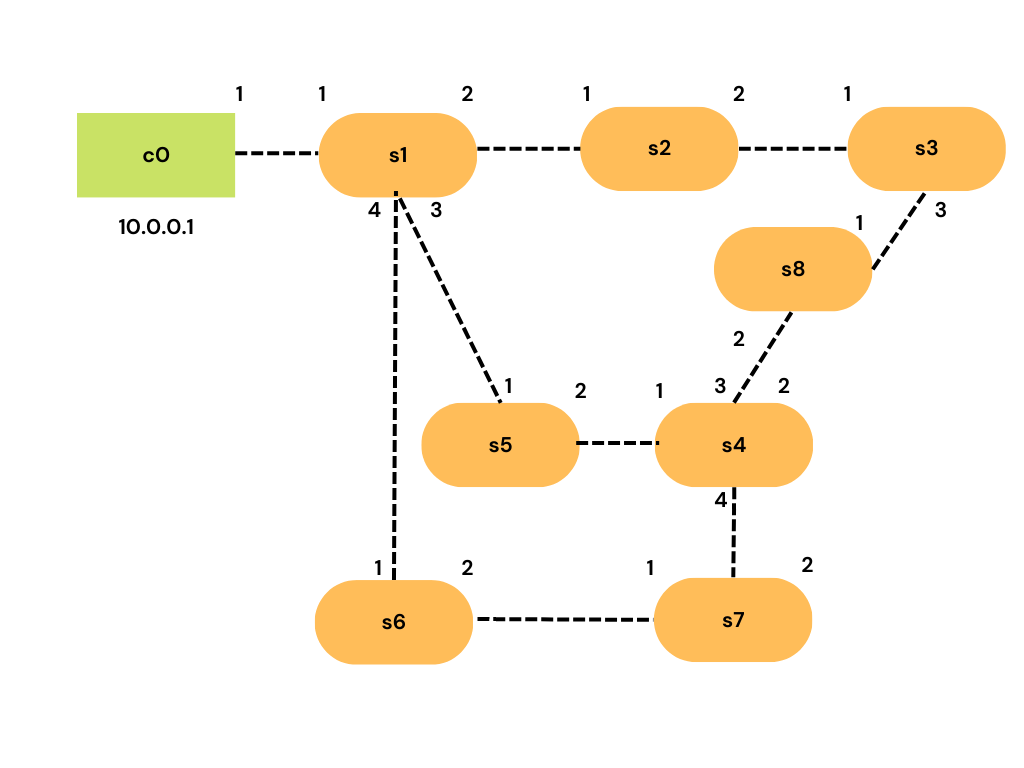
\includegraphics[width=12cm, keepaspectratio]{img/escenario1-1}
 		\caption{Primer escenario con un controlador}
 		\label{figura:escenario1-1c}
 	\end{figure}
 	
 	%Figura Escenario 1 con 2 controladores
 	\begin{figure}[H]
 		\centering
 		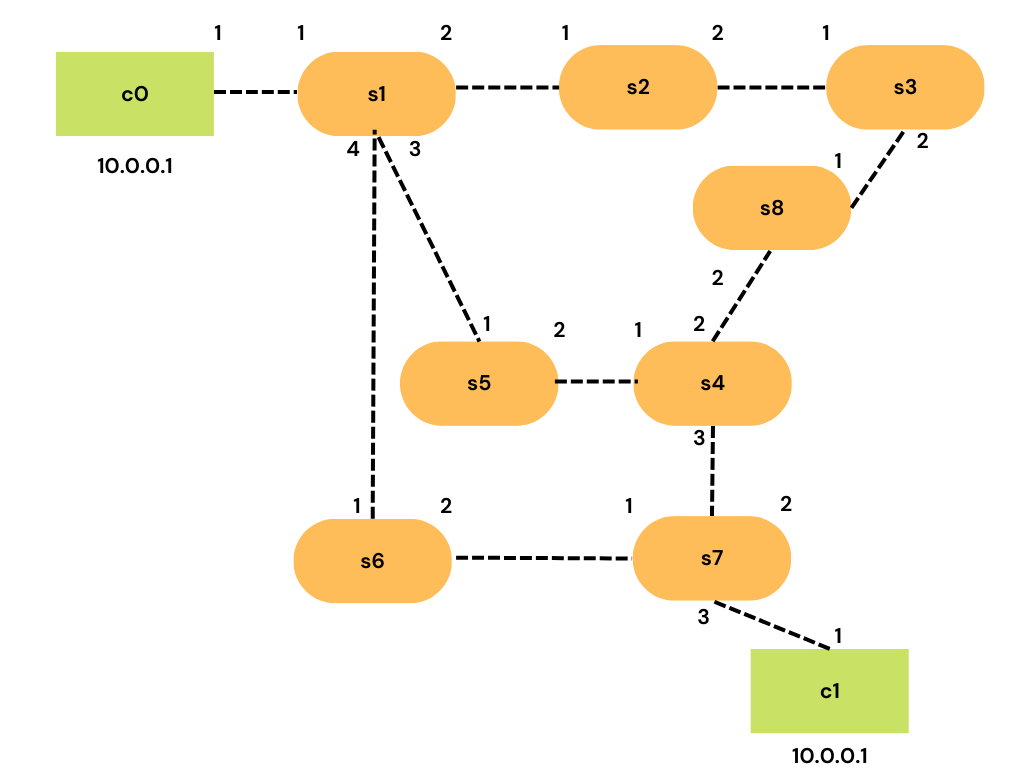
\includegraphics[width=12cm, keepaspectratio]{img/escenario1-2}
 		\caption{Primer escenario con 2 controladores}
 		\label{figura:escenario1-2c}
 		\vspace{-18pt}
 	\end{figure}
 	
 	En este escenario, vemos como desde el primer controlador al switch mas lejano, hay 4 saltos de switch. Al añadir un segundo controlador en el otro extremo del escenario, el switch mas lejano sería 3 saltos, por lo que ya vemos que deberíamos ver mejoría, pero tampoco se espera unos tiempos muy inferiores al mismo escenario con un controlador.
 	
 	Con estos resultados (~\ref{figura:comparativabucle4}), podemos confirmar que la agregación de nuevos controladores a un escenario reducirá los tiempos máximos de conexión. La media de mejora en este escenario es de 0.0546 segundos, siendo esto una mejora del 14.59 \% al añadir un controlador extra al escenario. 
 	Estos resultados coinciden con lo que se esperaba previamente, ya que hay una mejoría, pero no es demasiado grande con respecto al mismo escenario con un solo controlador.
 	
 	%Figura comparativa de tiempos en el primer escenario
 	\begin{figure}[H]
 		\centering
 		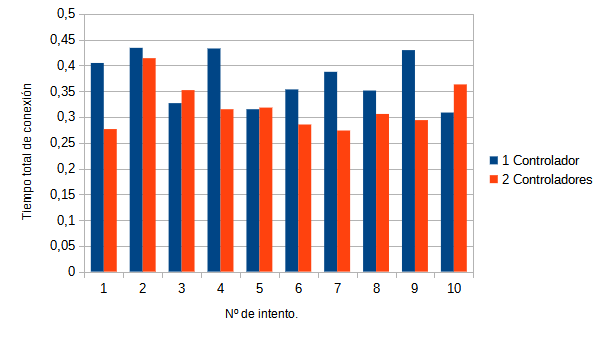
\includegraphics[width=16cm, keepaspectratio]{img/comparativabucle4}
 		\caption{Comparativa de tiempos en el primer escenario}
 		\label{figura:comparativabucle4}
 	\end{figure}
 	
 	%Figura comparativa de medias en el primer escenario
 	\begin{figure}[H]
 		\centering
 		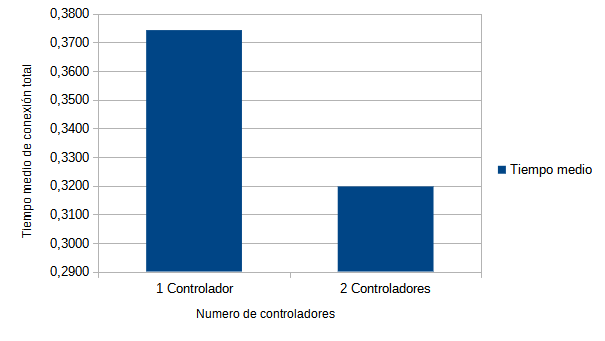
\includegraphics[width=12cm, keepaspectratio]{img/comparativamediasbucle}
 		\caption{Comparativa de media de tiempos en el primer escenario}
 		\label{figura:mediabucle4}
 	\end{figure}
 	
 	
 	Y como vemos en las siguientes gráficas, también hay bastante diferencia en la mediana y la varianza. Ya que al haber 2 controladores, es difícil que haya tiempos muy altos, de ahí que se reduzca la mediana y la varianza.
 	
 	%Figura comparativa de medianas en el primer escenario
 	\begin{figure}[H]
 		\centering
 		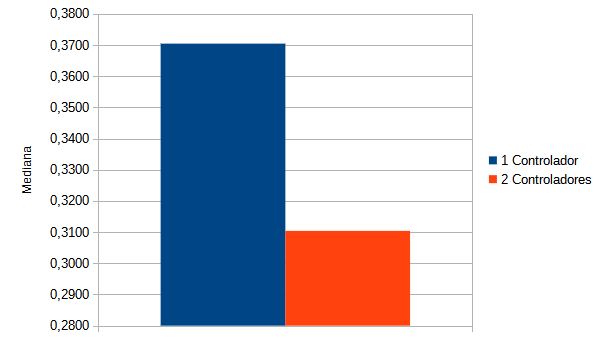
\includegraphics[width=12cm, keepaspectratio]{img/comparativamedianabucle}
 		\caption{Comparativa de medianas en el primer escenario}
 		\label{figura:medianabucle4}
 	\end{figure}
 	
 	%Figura comparativa de varianzas en el primer escenario
 	\begin{figure}[H]
 		\centering
 		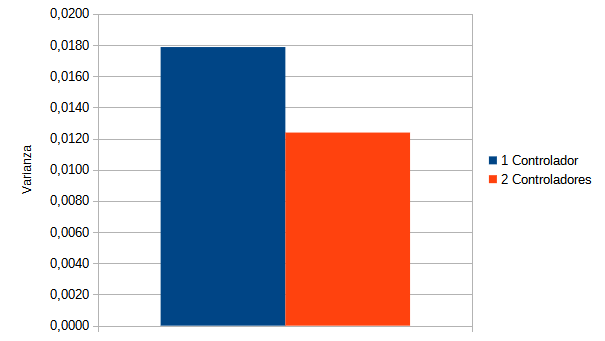
\includegraphics[width=12cm, keepaspectratio]{img/comparativavarianzabucle}
 		\caption{Comparativa de varianza de tiempos en el primer escenario}
 		\label{figura:varianzabucle4}
 	\end{figure}
 	
 	Con el objetivo de ilustrar como cambia el escenario al añadir un controlador extra, se van a comparar los dos experimentos, viendo como se han ido controlando los switches paso a paso.
 	
 	Para el caso de 1 controlador, los esquemas se han ido conectando de las siguientes formas:
 	
 	\begin{figure}[H]
 		\centering
 		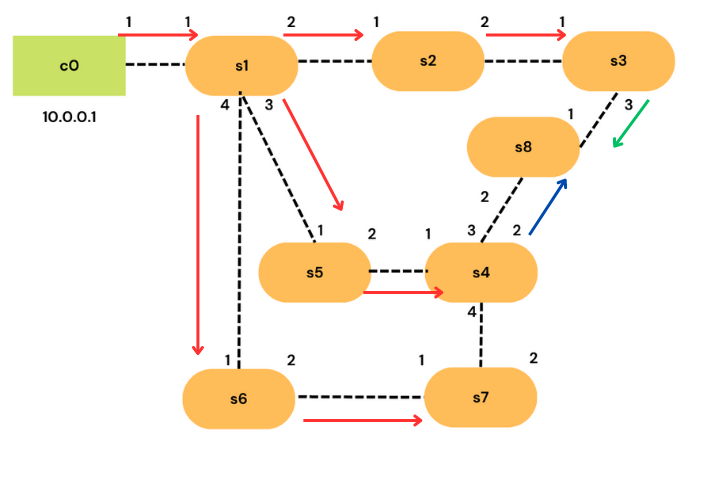
\includegraphics[width=12cm, keepaspectratio]{img/rutasEscenario1-1c}
 		\caption{Orden de conexión de los switches. El color rojo indica las conexiones con dirección comunes, quedando el color azul y verde para distinguir las diferencias entre rutas. \textcolor{blue}{1,}  \textcolor{green}{2}  \textcolor{blue}{,3, 4, 5, 6 ,7, 8,}  \textcolor{green}{9} \textcolor{blue}{,10}}
 		\label{figura:escenario1_1c_1}
 	\end{figure}
 	
 	Para el caso de 2 controladores, como era de esperar es bastante diferente, quedando así:
 	
 	\begin{figure}[H]
 		\centering
 		
 		\subfigure[Orden de conexión de los experimentos 1, 4]{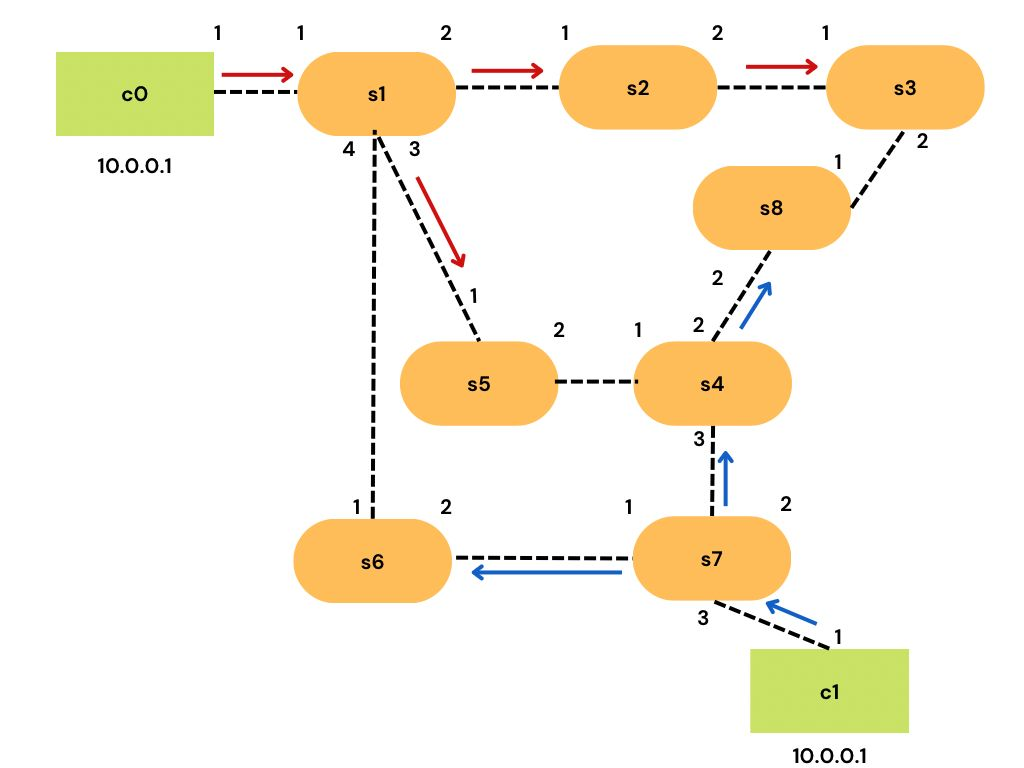
\includegraphics[width=0.45\textwidth]{img/escenario1_2c_1}}
 		\hfill
 		\subfigure[Orden de conexión de los experimentos 2, 9]{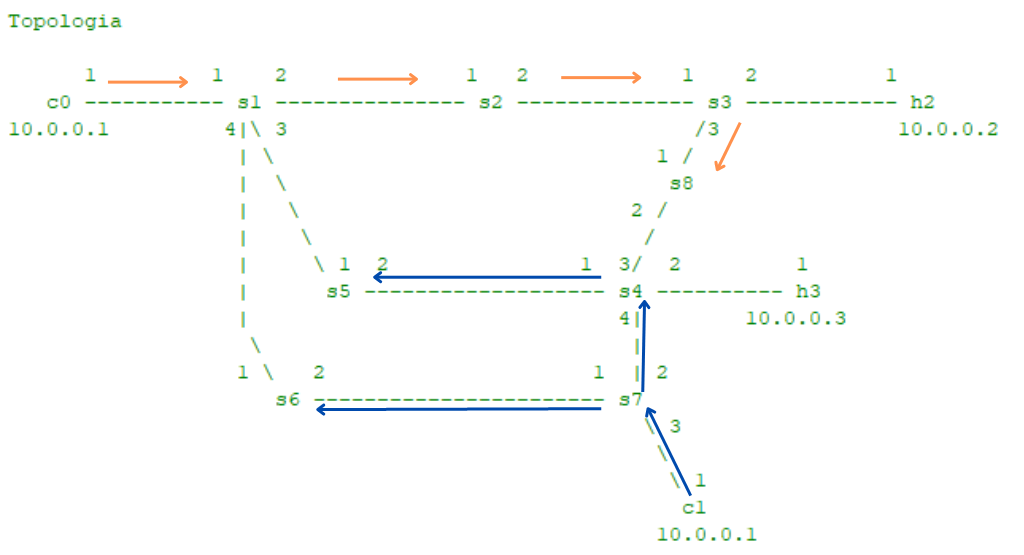
\includegraphics[width=0.45\textwidth]{img/escenario1_2c_2}}
 		\hfill
 		\vspace{10pt} % Ajusta el espacio vertical entre las filas
 		\subfigure[Orden de conexión del experimento 3]{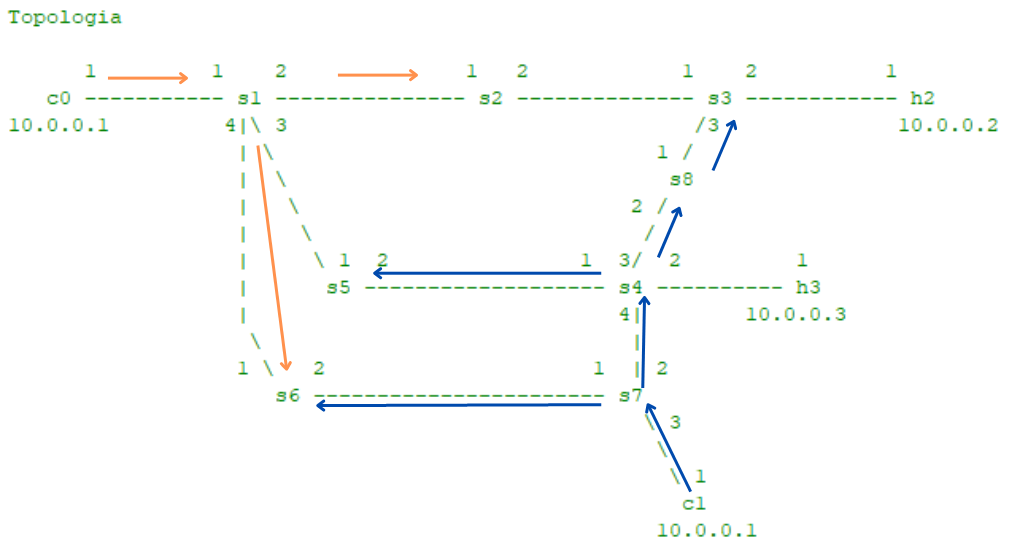
\includegraphics[width=0.45\textwidth]{img/escenario1_2c_3}}
 		\subfigure[Orden de conexión del experimento 5]{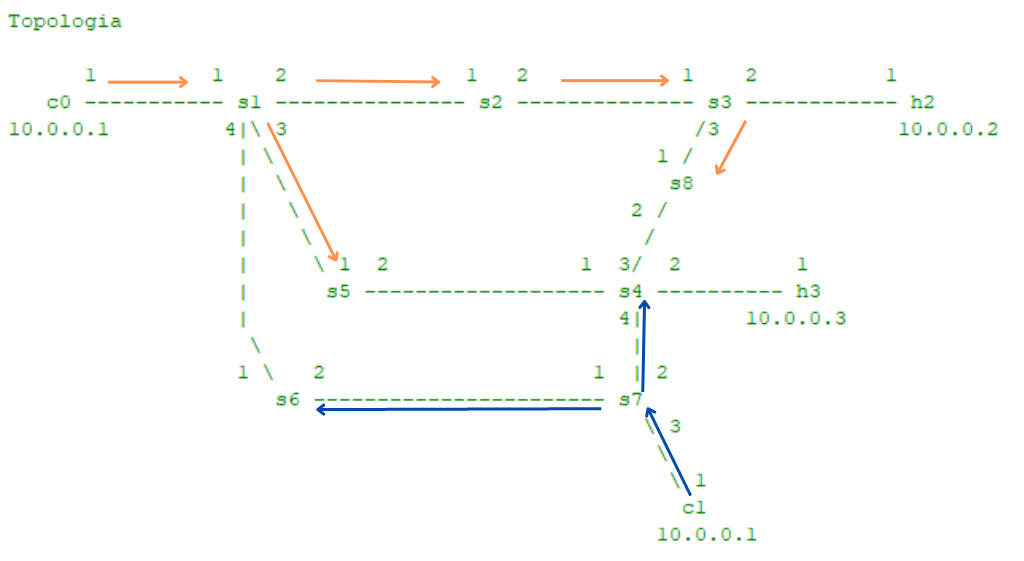
\includegraphics[width=0.45\textwidth]{img/escenario1_2c_4}}
 		\hfill
 		\vspace{10pt} % Ajusta el espacio vertical entre las filas
 		
 	
 		\subfigure[Orden de conexión del experimento 6]{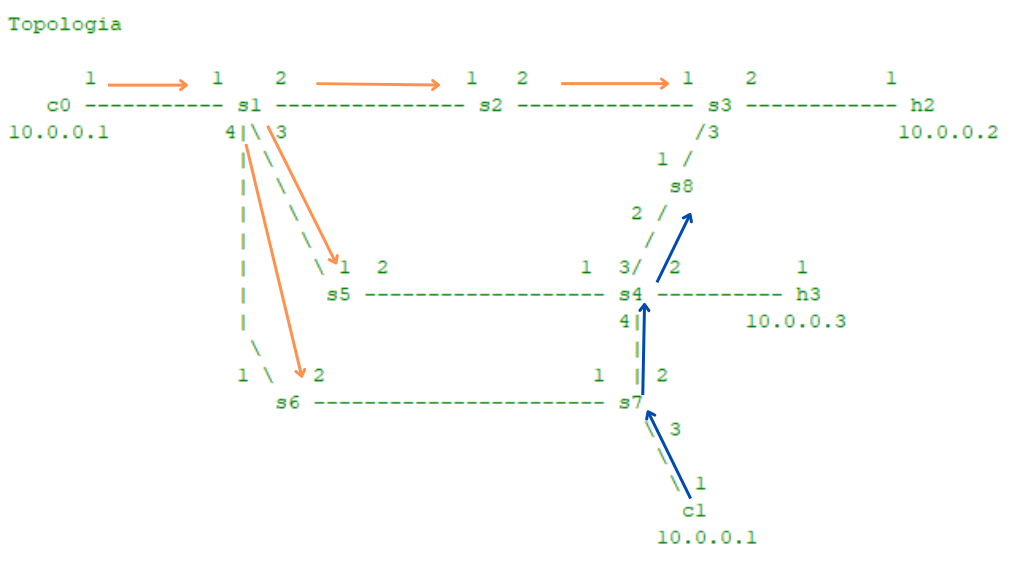
\includegraphics[width=0.45\textwidth]{img/escenario1_2c_5}}
 		\hfill
 		\subfigure[Orden de conexión del experimento 7]{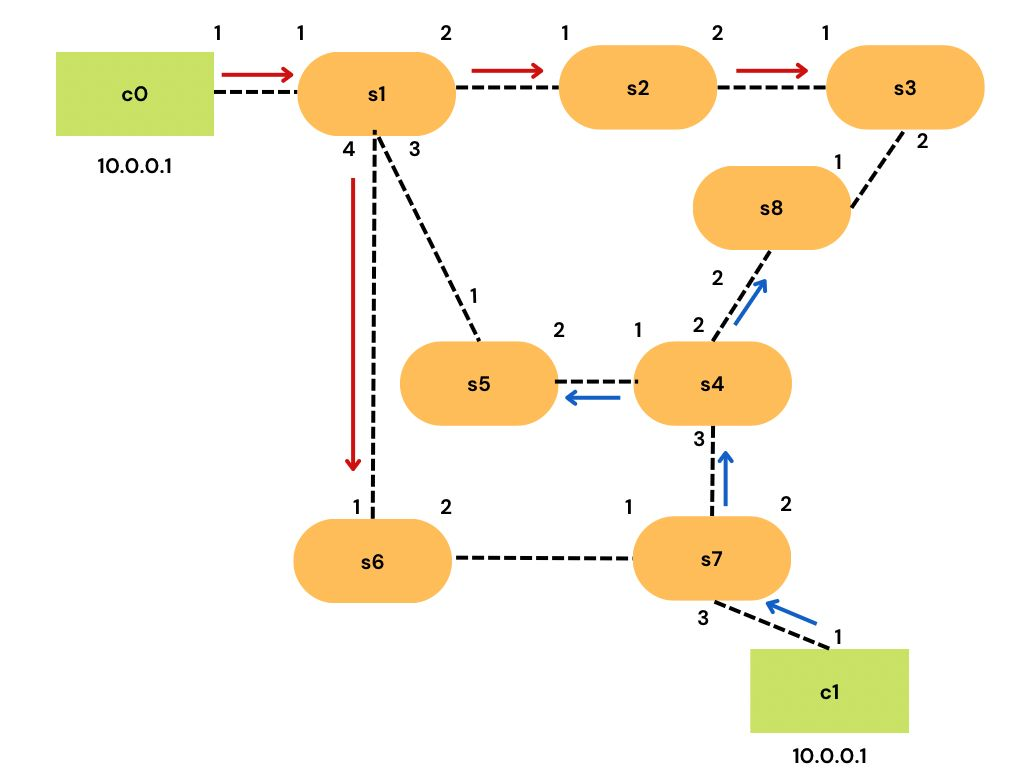
\includegraphics[width=0.45\textwidth]{img/escenario1_2c_6}}
 		
 		\vspace{10pt} % Ajusta el espacio vertical entre las filas
 		\subfigure[Orden de conexión del experimento 8]{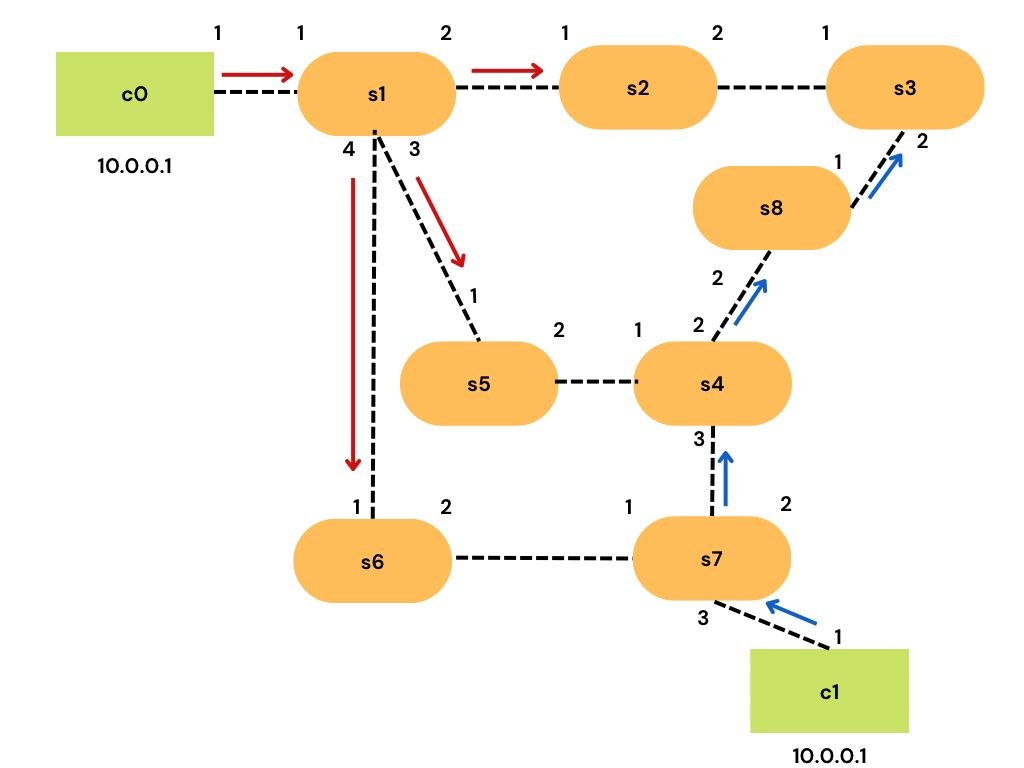
\includegraphics[width=0.45\textwidth]{img/escenario1_2c_7}}
 		\hfill
 		\subfigure[Orden de conexión del experimento 10]{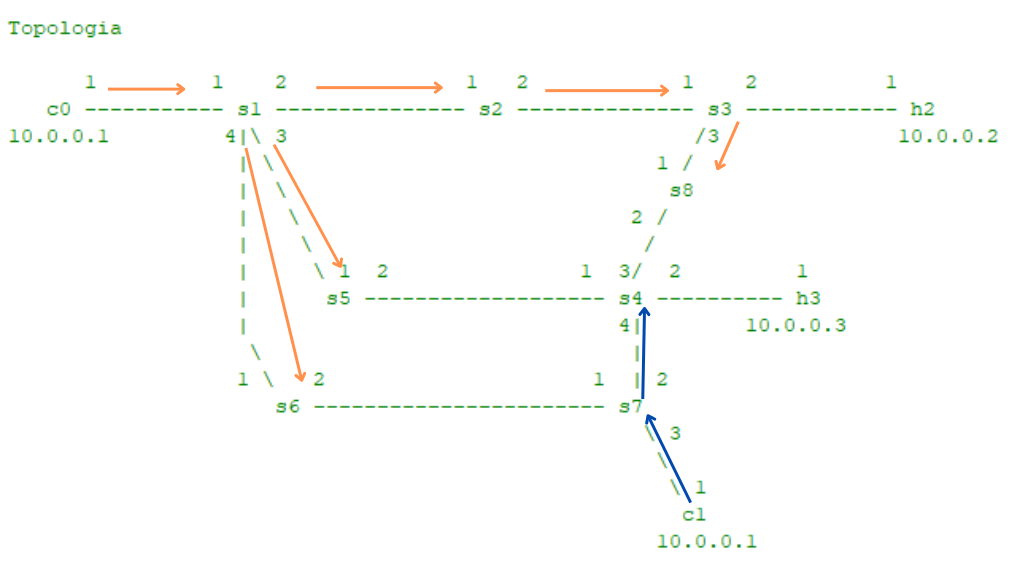
\includegraphics[width=0.45\textwidth]{img/escenario1_2c_8}}
 		
 		\caption{Conjunto de 8 imágenes}
 	\end{figure}
 	
 	Como podemos comprobar, pese a haber 10 experimentos, hemos podido ver 8 formas diferentes de controlar los switches. Algo que muestra la flexibilidad que tiene Periplus a la hora de realizar conexiones, que para este caso no es necesario, pero para escenarios mucho mas grandes nos será muy útil.
 	
 	De estos datos, además podemos comprobar el reparto de switches que se ha ido haciendo por controlador. Siendo bastante equilibrado, algo que de nuevo nos muestra la utilidad de Periplus.
 	
 	\begin{figure}[H]
 		\centering
 		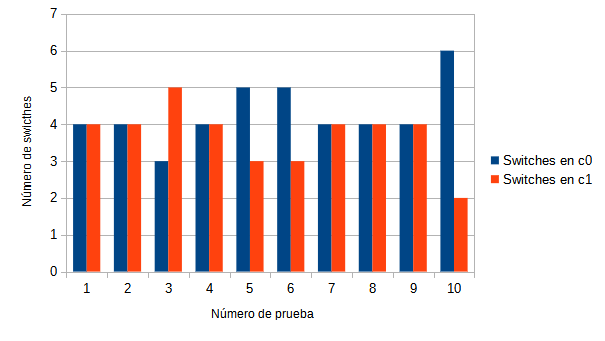
\includegraphics[width=16cm, keepaspectratio]{img/switchesporcontrollerescenario1}
 		\caption{Número de switches por controlador.}
 		\label{figura:switchesporcontrollerescenario1}
 	\end{figure}
 	
 	
 	
 	\clearpage
 	\section{Escenario 2}
 	
 	En este caso, se analizará un escenario más complejo ~\ref{figura:escenario2-1c} y el mismo escenario con 4 controladores en vez de 1 ~\ref{figura:escenario2-4c}.
 	
 	En este escenario se espera una mejora muy superior a la vista en el primer escenario, ya que en el ejemplo con 1 controlador hay hasta 6 saltos hasta el switch mas lejano, y con 4 controladores se reduce a 3, por lo que a priori podríamos esperar una mejora bastante superior a la obtenida en el primer escenario.
 	
 	\begin{figure}[H]
 		\centering
 		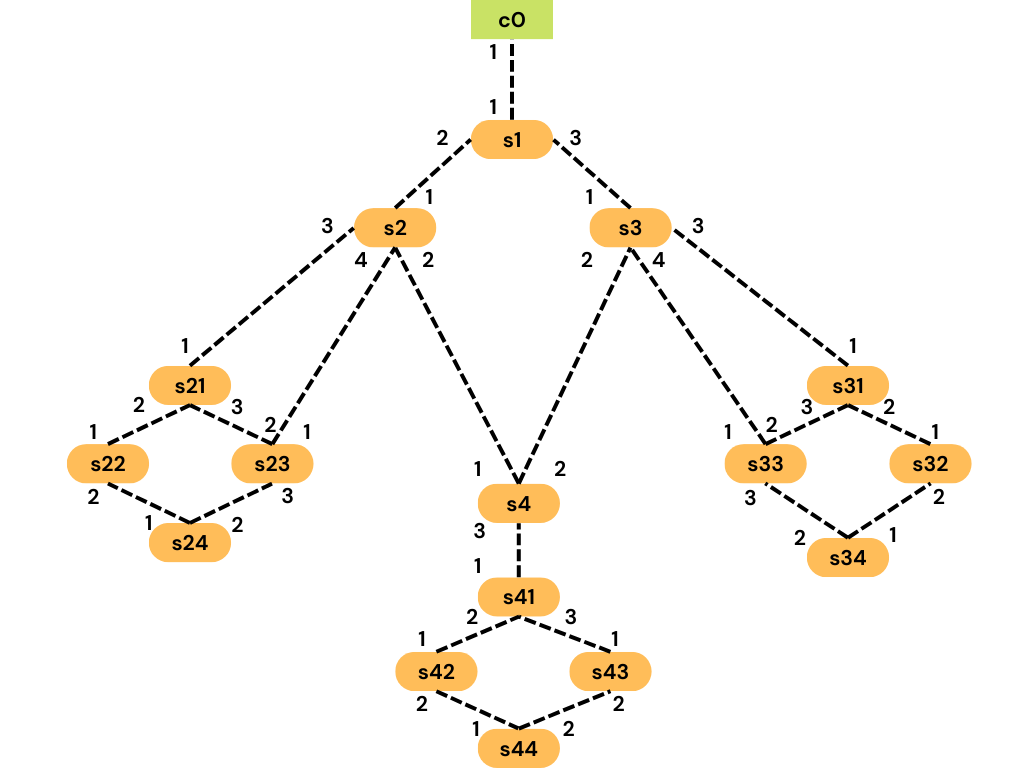
\includegraphics[width=14cm, keepaspectratio]{img/escenario2-1}
 		\caption{Segundo escenario con 1 controlador}
 		\label{figura:escenario2-1c}
 	\end{figure}
 	
 	\begin{figure}[H]
 		\centering
 		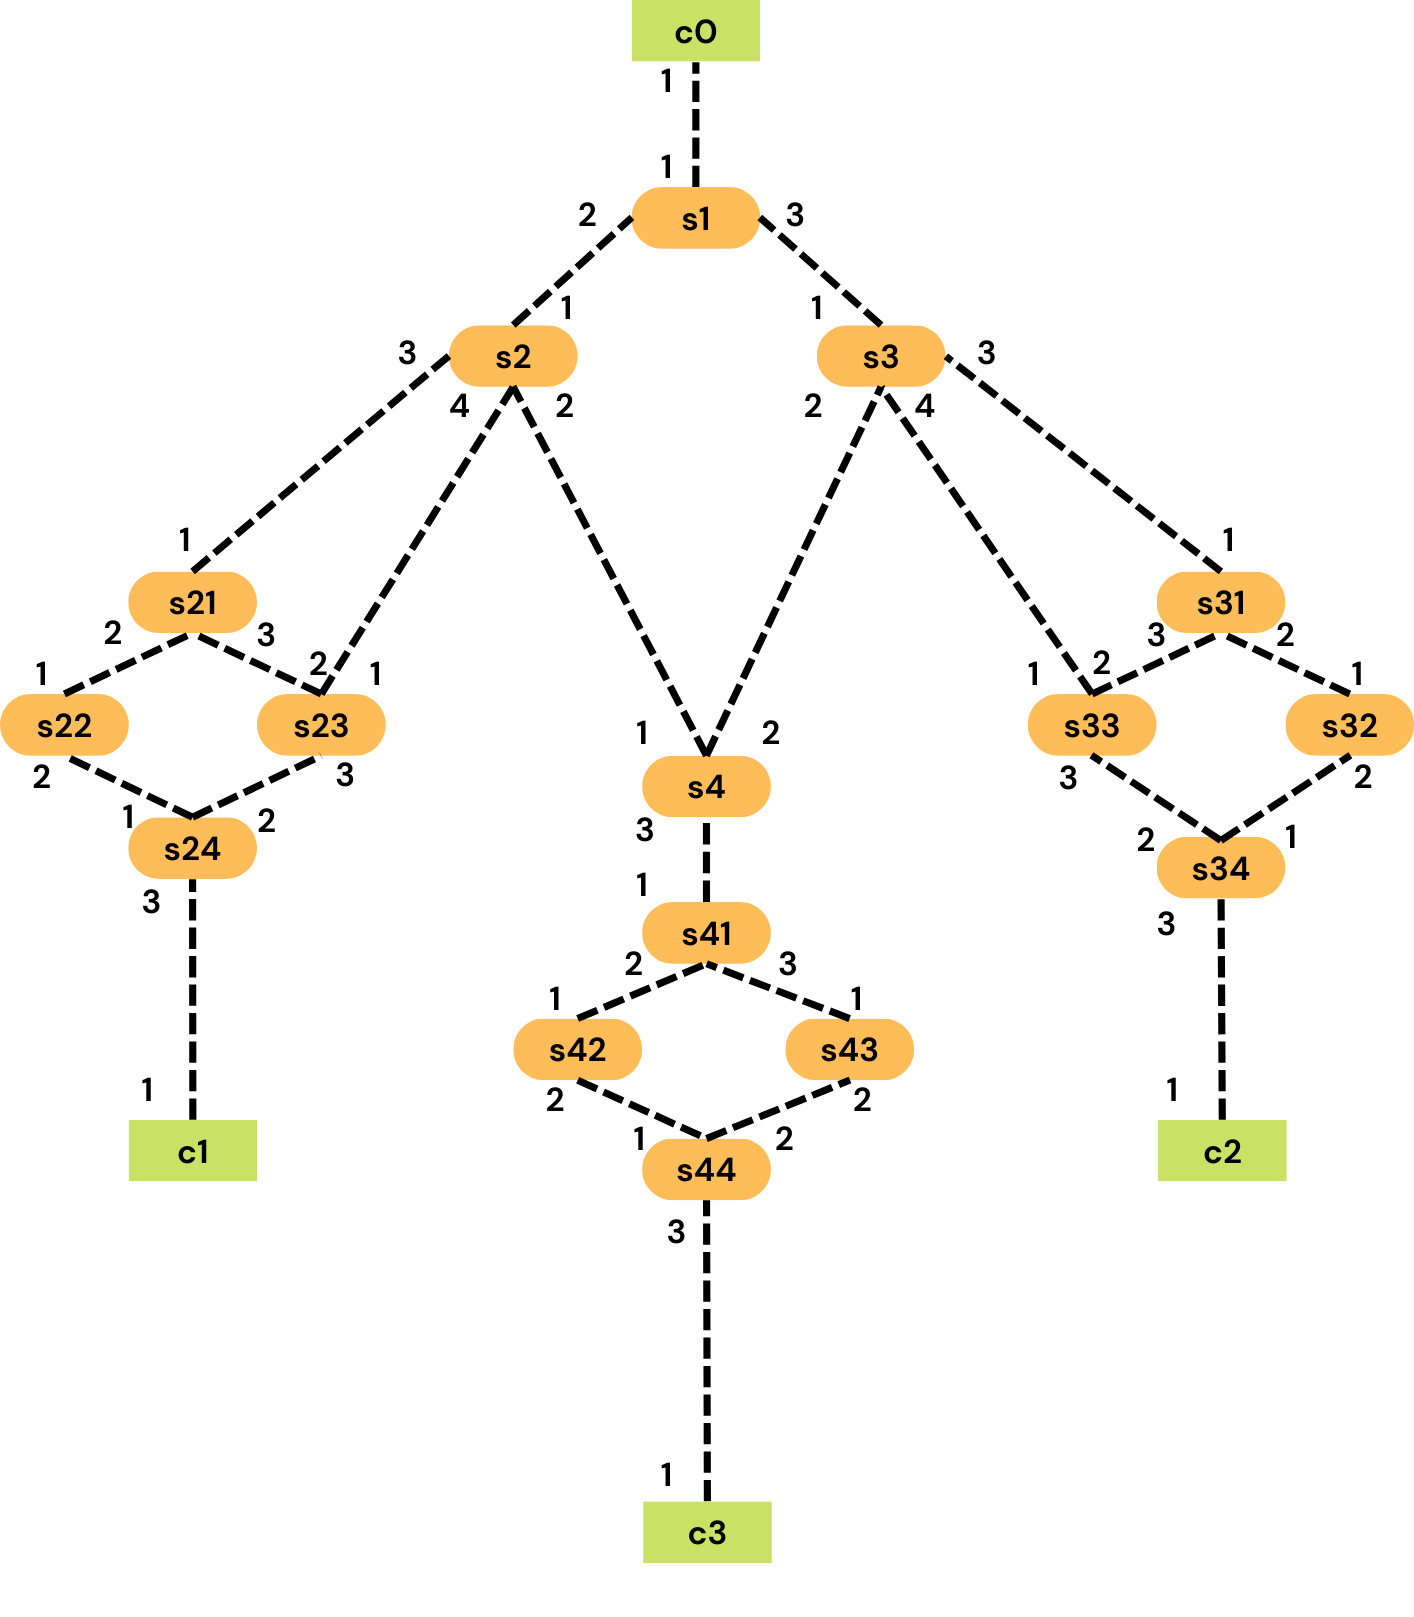
\includegraphics[width=14cm, keepaspectratio]{img/escenario2-2}
 		\caption{Segundo escenario con 4 controladores}
 		\label{figura:escenario2-4c}
 	\end{figure}
 	
 	Con estos resultados (~\ref{figura:comparativamesh}, ~\ref{figura:mediamesh} ), podemos confirmar lo visto en el escenario 1 y lo que esperábamos antes de ver los resultados, ya que además en este escenario, al ser mas grande y complejo, la disminución es mas notoria, ya que el tiempo máximo de conexión en los switches se ha reducido en 0.1464 segundos, siendo el sistema un 26.28 \% mas rápido con 4 controladores que con 1.
 	
 	%Figura comparativa de tiempos en el segundo escenario
 	\begin{figure}[H]
 		\centering
 		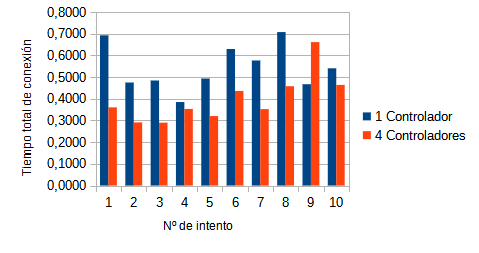
\includegraphics[width=16cm, keepaspectratio]{img/comparativamesh}
 		\caption{Comparativa de tiempos en el segundo escenario}
 		\label{figura:comparativamesh}
 	\end{figure}
 	
 	
 	%Figura comparativa de medias en el segundo escenario
 	\begin{figure}[H]
 		\centering
 		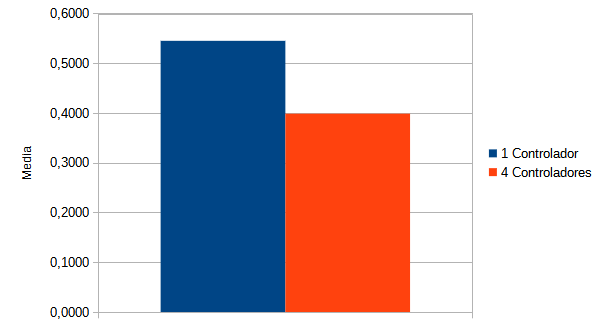
\includegraphics[width=12cm, keepaspectratio]{img/comparativamediamesh}
 		\caption{Comparativa de media de tiempos en el segundo escenario}
 		\label{figura:mediamesh}
 	\end{figure}
 	
 	
 	Y como vemos en las siguientes gráficas, también hay bastante diferencia en la mediana y la varianza. Ya que al haber 4 controladores, es difícil que haya tiempos muy altos, de ahí que se reduzca la mediana y la varianza.
 	
 	\begin{figure}[H]
 		\centering
 		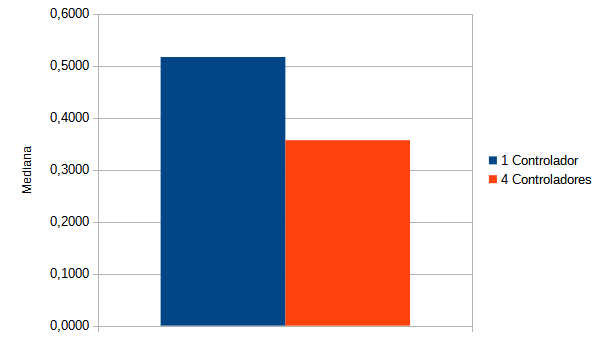
\includegraphics[width=12cm, keepaspectratio]{img/comparativamedianamesh}
 		\caption{Comparativa de medianas en el segundo escenario}
 		\label{figura:medianamesh}
 	\end{figure}
 	
 	\begin{figure}[H]
 		\centering
 		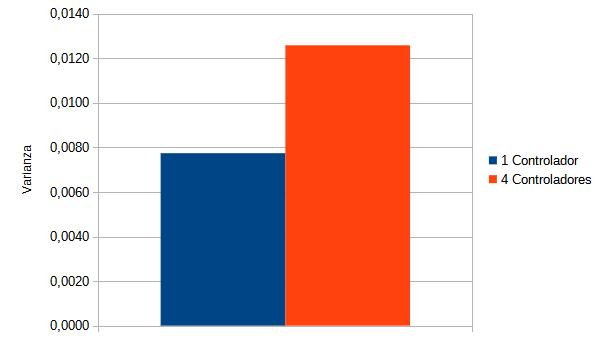
\includegraphics[width=12cm, keepaspectratio]{img/comparativavarianzamesh}
 		\caption{Comparativa de varianza de tiempos en el segundo escenario}
 		\label{figura:varianzamesh}
 	\end{figure}
 	
 	\vspace{10pt} 
 	
 	Además, hemos comprobado que por lo general el reparto de switches entre los controladores se ha realizado de forma bastante equitativa. El reparto de los últimos experimentos se asocian a fallo de la máquina al realizar los experimentos, algo que ha ocurrido en los escenarios mas grandes debido a la gran carga de trabajo que tenía el ordenador al realizar las simulaciones. Pero ya con el primer reparto de switches, que ha sido equitativo, vemos que la tecnología funciona perfectamente y hace lo que se espera.
 	
 	
 	\begin{figure}[H]
 		\centering
 		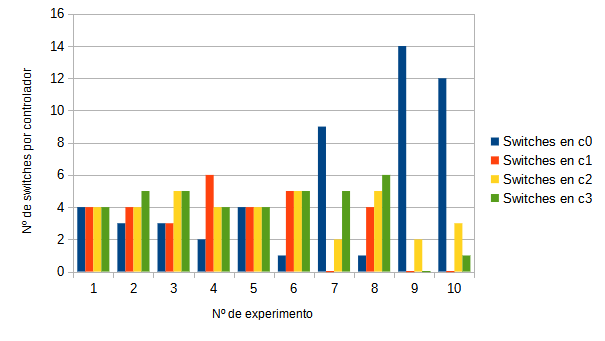
\includegraphics[width=16cm, keepaspectratio]{img/switchesporcontrollermesh}
 		\caption{Número de switches por controlador.}
 		\label{figura:switchesporcontrollermesh}
 	\end{figure}
 	
 	
 	\clearpage
 	\section{Escenario 3}
 	 
 	A continuación, se llevará a cabo un análisis de un escenario con caminos más complejos y largos ~\ref{figura:b4_1} y el mismo escenario con 2 controladores en vez de 1 ~\ref{figura:b4_2}, para ver cómo reacciona Periplus en este caso.
 	En el escenario con un controlador, vemos que el switch mas lejano está a 4 saltos, mientras que el escenario con dos controladores el switch mas lejano está a 3 saltos. Lo curioso de este escenario es la gran cantidad de conexiones entre switches que hay, y que el segundo controlador se coloca en el extremo mas lejano, pero lejos de otra gran parte de los switches.
 	
 	%Figura comparativa de tiempos en el tercer escenario
 	\begin{figure}[H]
 		\centering
 		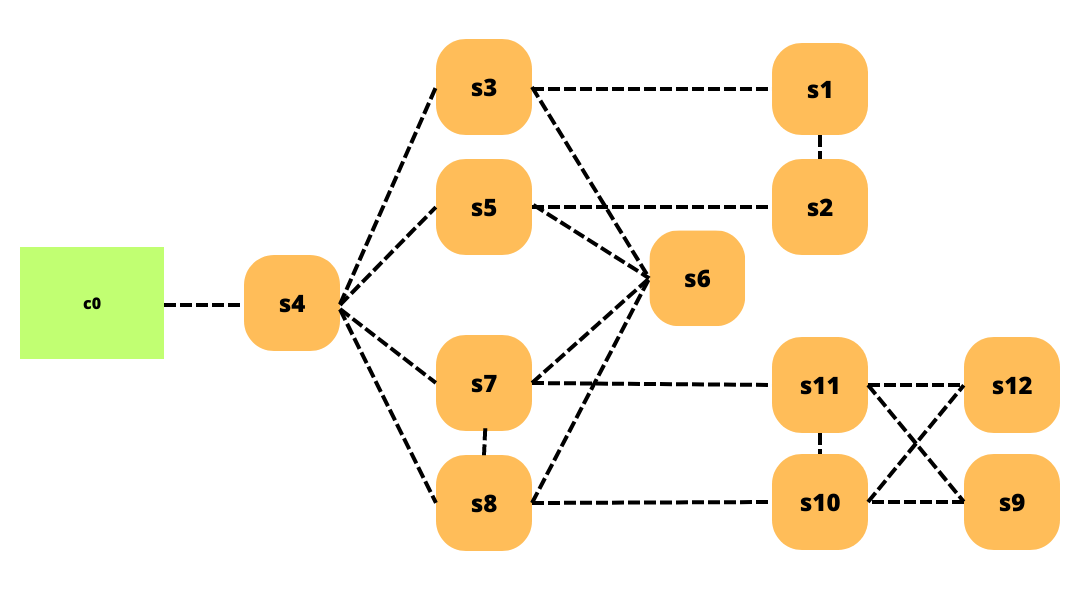
\includegraphics[width=14cm, keepaspectratio]{img/b4_1}
 		\caption{Tercer escenario con 1 controlador}
 		\label{figura:b4_1}
 	\end{figure}
 	
 	%Figura comparativa de medias en el tercer escenario
 	\begin{figure}[H]
 		\centering
 		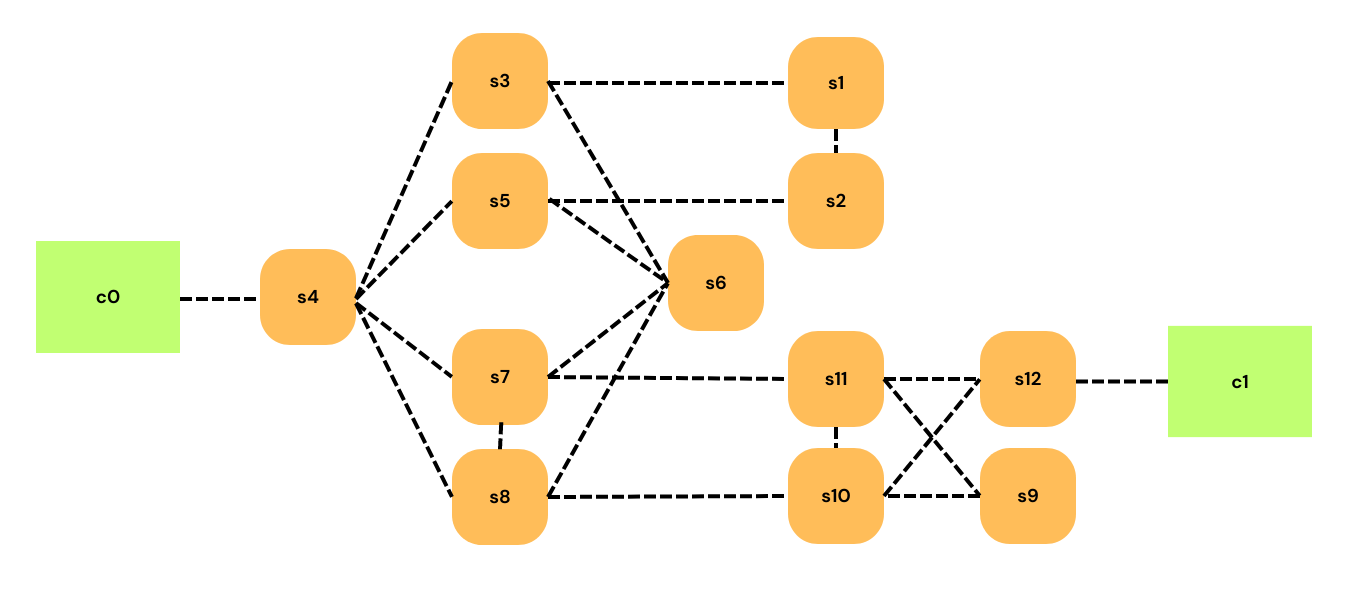
\includegraphics[width=14cm, keepaspectratio]{img/b4_2}
 		\caption{Tercer escenario con 2 controladores}
 		\label{figura:b4_2}
 	\end{figure}
 	
 	Con estos resultados(~\ref{figura:comparativab4}, ~\ref{figura:mediab4}), podemos confirmar lo visto en los anterior escenarios, ya que además en este escenario, al ser mas grande y complejo, la disminución es mas notoria, ya que el tiempo máximo de conexión en los switches se ha reducido en 0.168 segundos, siendo el sistema un 47.19 \% mas rápido con 2 controladores que con 1.
 	
 	Además comparando tiempos, se empieza a ver una tendencia, que cuantos mas saltos entre switches se reduzcan, mas efectivo es el circuito.
 	
 	\begin{figure}[H]
 		\centering
 		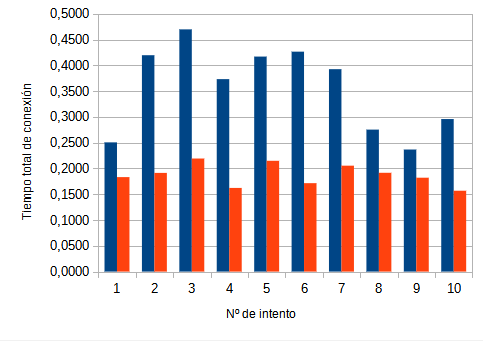
\includegraphics[width=12cm, keepaspectratio]{img/comparativaescenario3}
 		\caption{Comparativa de tiempos en el tercer escenario}
 		\label{figura:comparativab4}
 	\end{figure}
 	
 	
 	
 	\begin{figure}[H]
 		\centering
 		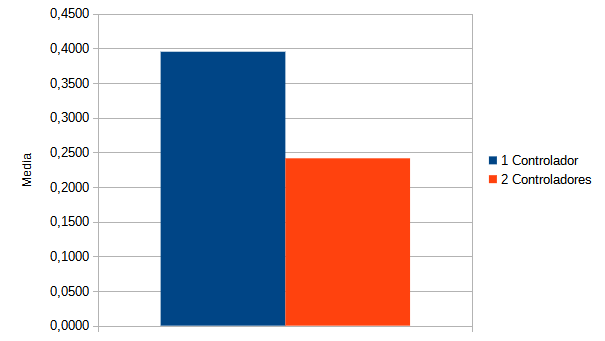
\includegraphics[width=12cm, keepaspectratio]{img/comparativamediaescenario3}
 		\caption{Comparativa de media de tiempos en el tercer escenario}
 		\label{figura:mediab4}
 	\end{figure}
 	
 	Y como vemos en las siguientes gráficas, también hay bastante diferencia en la mediana y la varianza. Ya que al haber 2 controladores y tanta conexión, es difícil que haya tiempos muy altos, de ahí que se reduzca la mediana y sobretodo la varianza.
 	
 	
 	\begin{figure}[H]
 		\centering
 		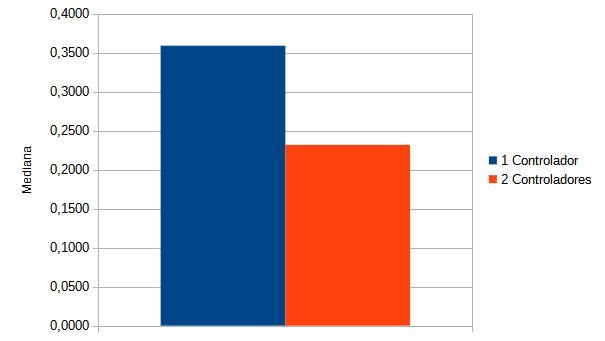
\includegraphics[width=12cm, keepaspectratio]{img/comparativamedianaescenario3}
 		\caption{Comparativa de medianas en el tercer escenario}
 		\label{figura:medianab4}
 	\end{figure}
 	
 	\begin{figure}[H]
 		\centering
 		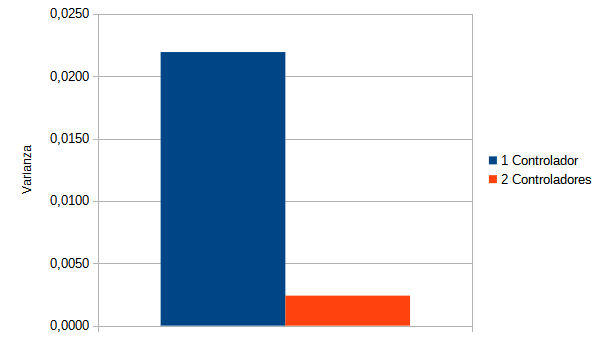
\includegraphics[width=12cm, keepaspectratio]{img/comparativavarianzaescenario3}
 		\caption{Comparativa de varianza de tiempos en el tercer escenario}
 		\label{figura:varianzab4}
 	\end{figure}
 	
 	\clearpage
 	Además, hemos comprobado que por lo general el reparto de switches entre los controladores se ha realizado de forma previsible y como se intuía al principio, el primer controlador tiene mas switches conectados en cada experimento, debido a que tiene una mayor cantidad de switches mas cerca que el segundo controlador.
 	
 	
 	\begin{figure}[H]
 		\centering
 		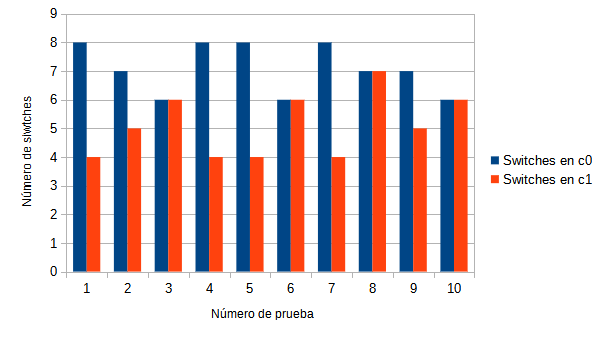
\includegraphics[width=16cm, keepaspectratio]{img/switchesporcontrollerescenario3}
 		\caption{Número de switches por controlador.}
 		\label{figura:switchesporcontrollerb4}
 	\end{figure}
	
	\clearpage
	\section{Escenario 4}
	
	En este último experimento y a diferencia de los escenarios anteriores, se realizará una tercera comparación, ya que estudiaremos un escenario con uno, dos, y cuatro controladores, para comprobar cómo cambia en función de cada caso.
	Serán los escenarios ~\ref{figura:e4_1}, el mismo escenario con 2 controladores ~\ref{figura:e4_2} y con 4 controladores ~\ref{figura:e4_3} para ver como reacciona OpenFlow en este caso.
	
	En este escenario, el numero de saltos no va a disminuir, ya que se va a mantener la misma distancia máxima entre los controladores y los switches mas alejados, pero se esperan tiempos mas bajos debido a que el reparto de trabajo se va a dividir por 2 y 4 respectivamente.
	
	\begin{figure}[H]
		\centering
		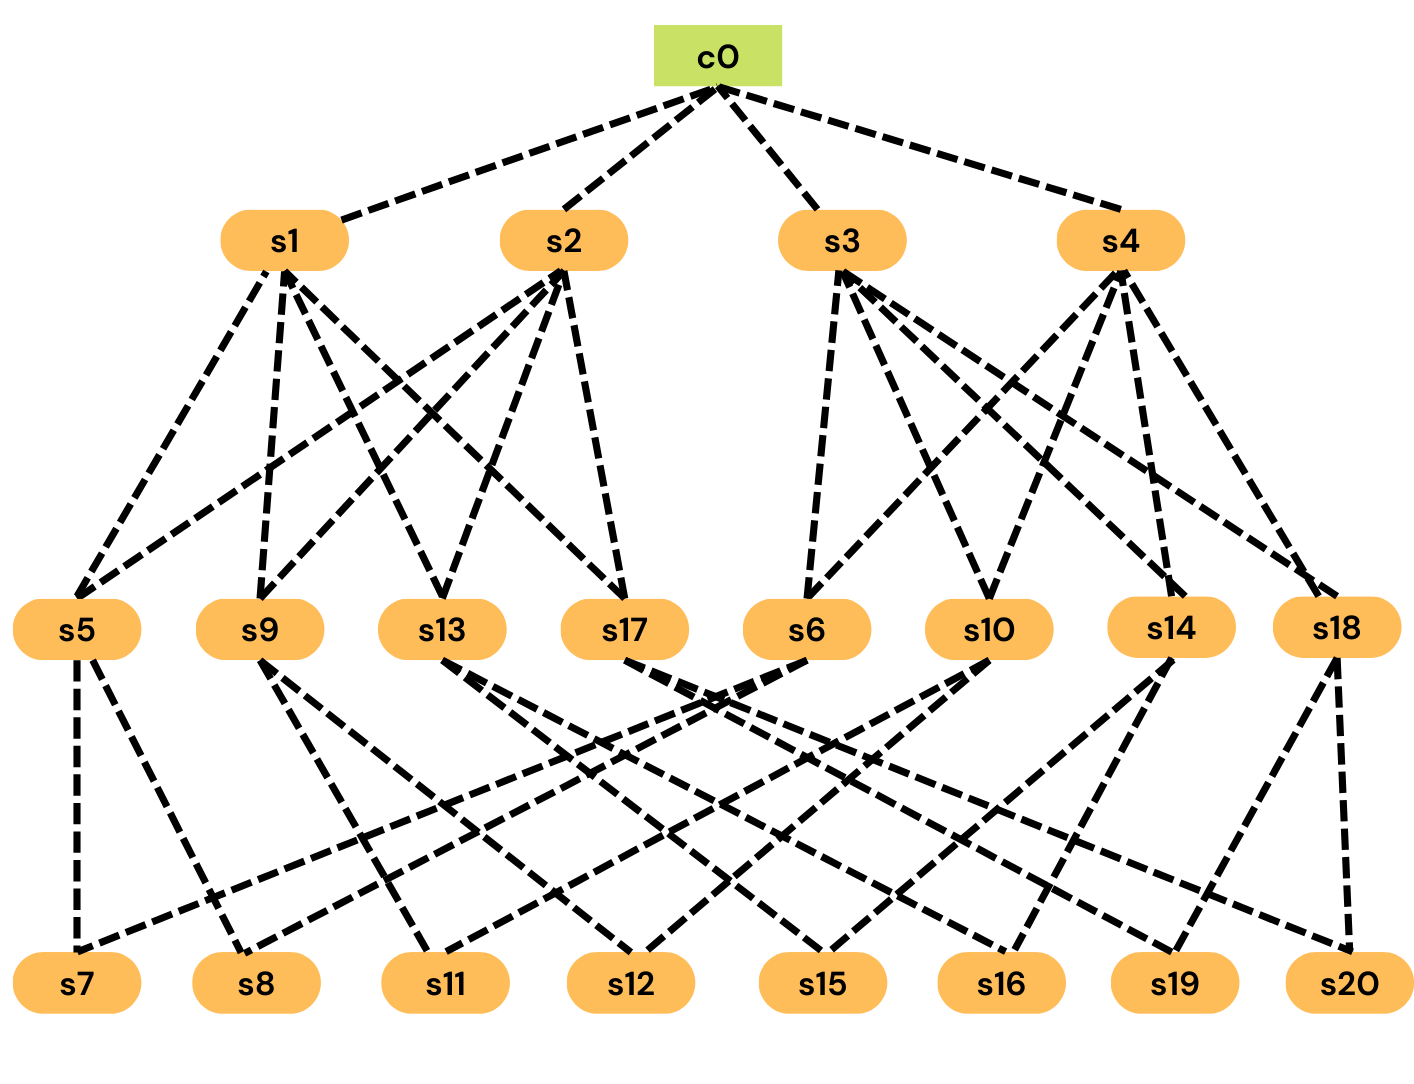
\includegraphics[width=16cm, keepaspectratio]{img/e4_1}
		\caption{Cuarto escenario con 1 controlador}
		\label{figura:e4_1}
	\end{figure}
	
	\begin{figure}[H]
		\centering
		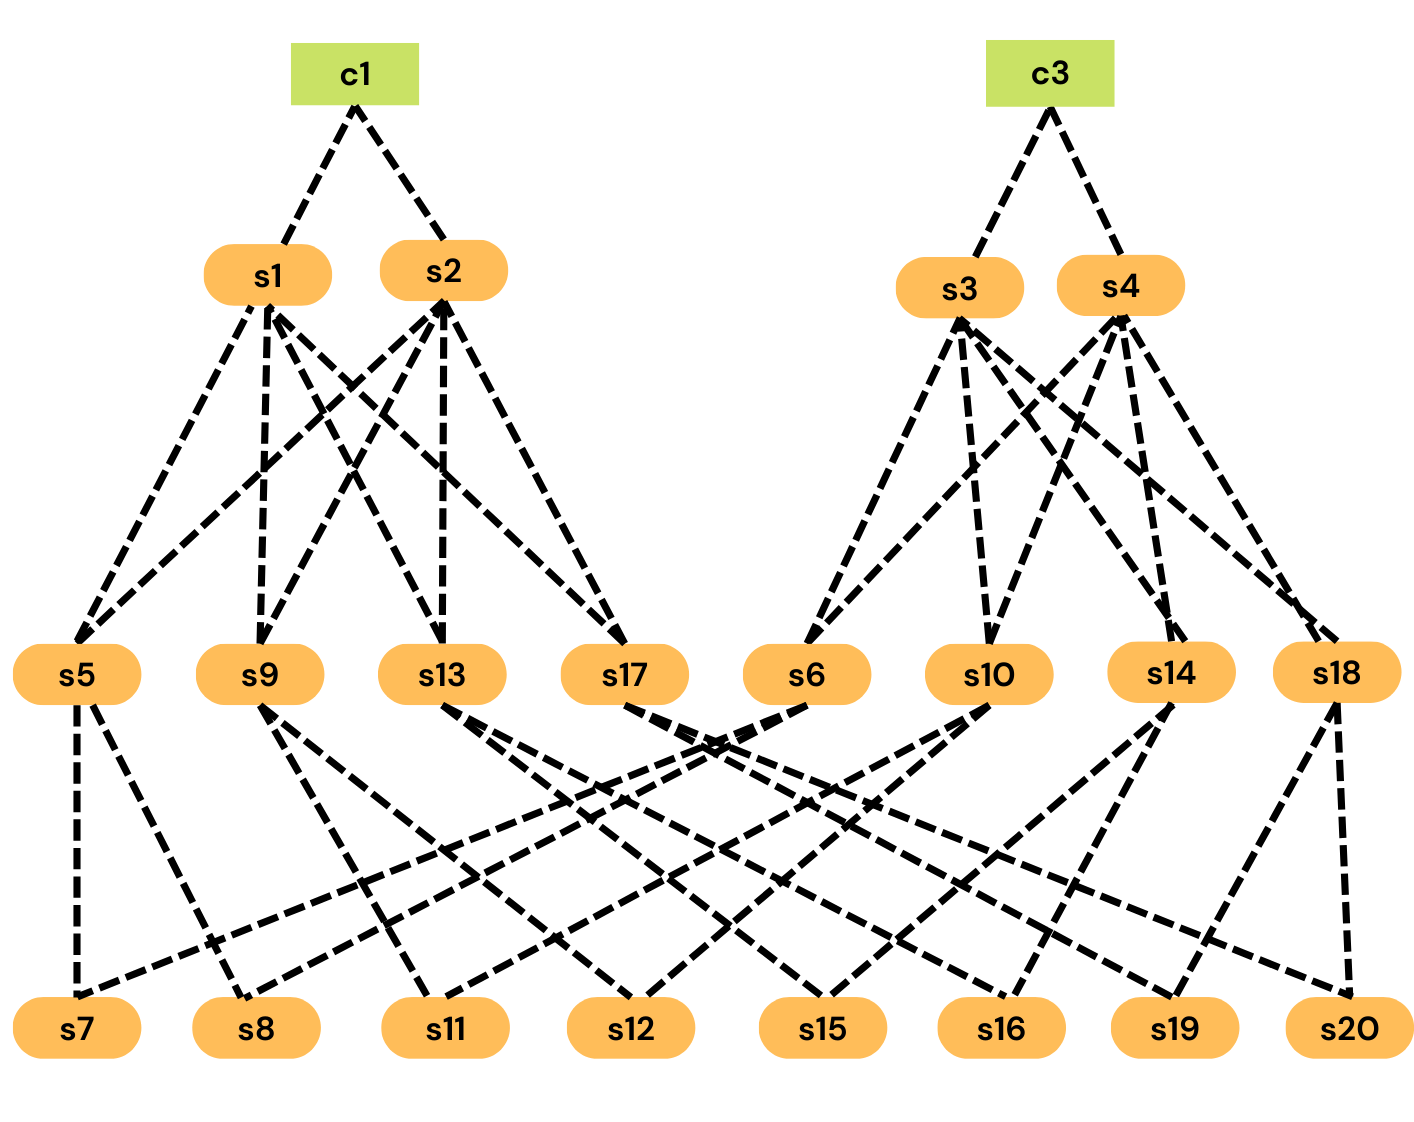
\includegraphics[width=13cm, keepaspectratio]{img/e4_2}
		\caption{Cuarto escenario con 2 controladores}
		\label{figura:e4_2}
	\end{figure}
	
	
	\begin{figure}[H]
		\centering
		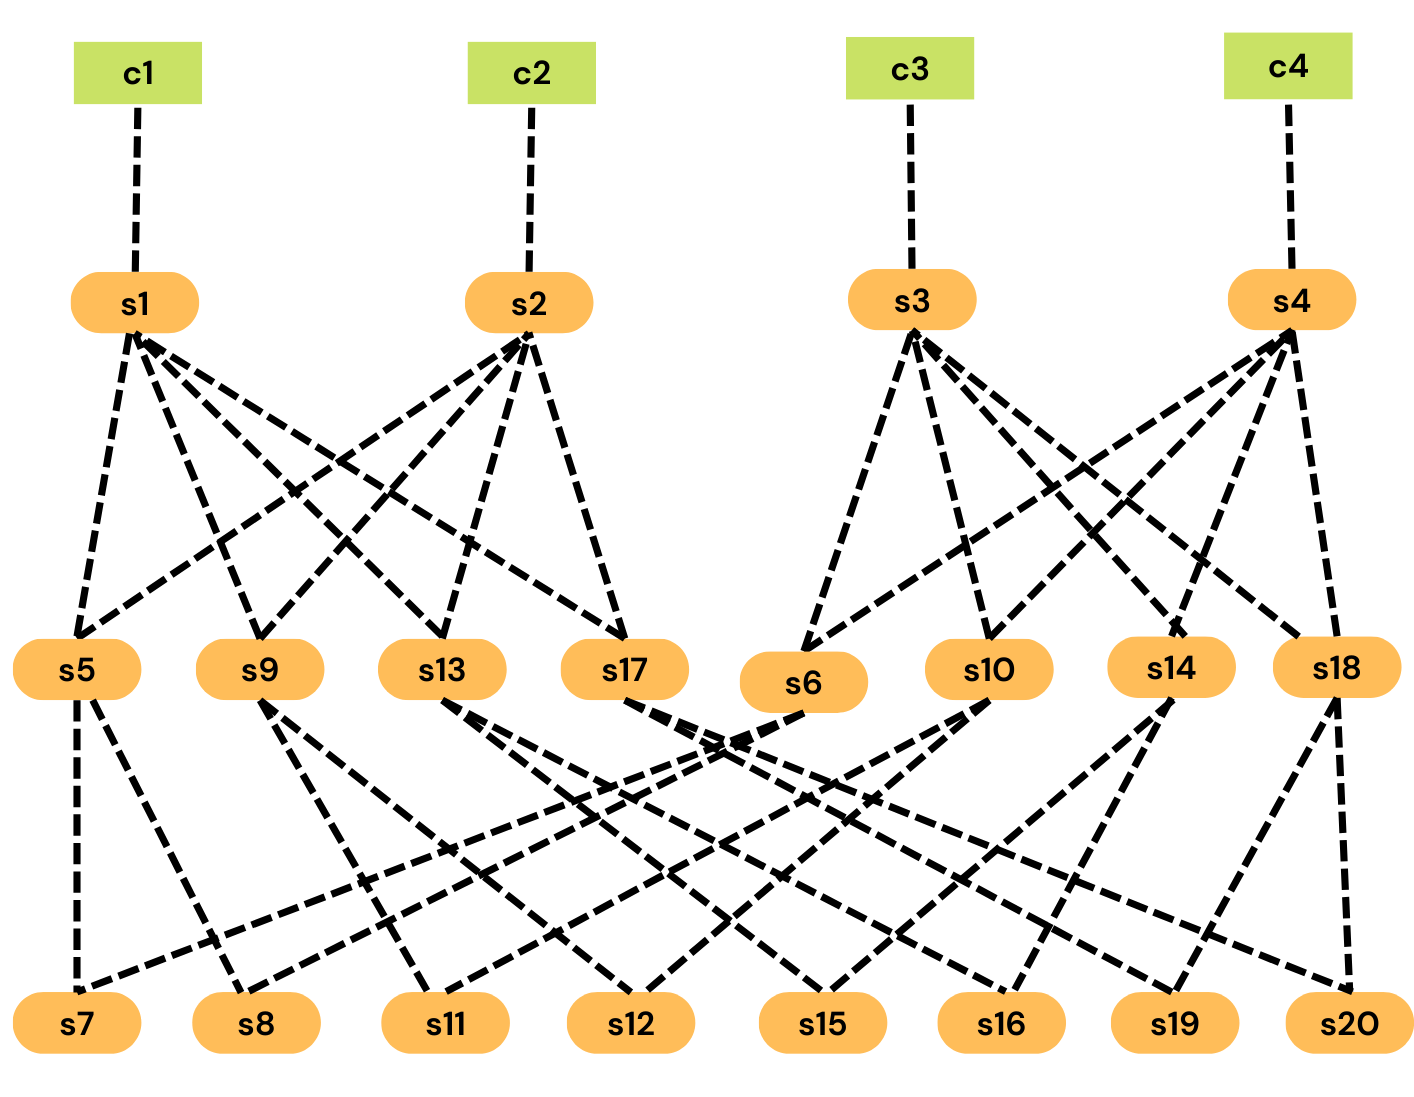
\includegraphics[width=13cm, keepaspectratio]{img/e4_3}
		\caption{Cuarto escenario con 4 controladores}
		\label{figura:e4_3}
	\end{figure}
	
En estas tablas(~\ref{figura:comparativaescenario4}, ~\ref{figura:mediaescenario4}), vemos la comparación del escenario con 1 y 2 controladores en tiempos y mediaqs podemos confirmar lo visto en los anterior escenarios, ya que además en este escenario, al ser mas grande y complejo, la disminución es mas notoria, ya que el tiempo máximo de conexión en los switches se ha reducido en 0.168 segundos, siendo el sistema un 47.19 \% mas rápido con 2 controladores que con 1. Teniendo en cuenta que la carga de trabajo se ha repartido entre 2, podemos observar que para escenarios complejos, cuantos mas controladores haya, mucho más rápida será la configuración de los switches.
		
		
	
	\begin{figure}[H]
		\centering
		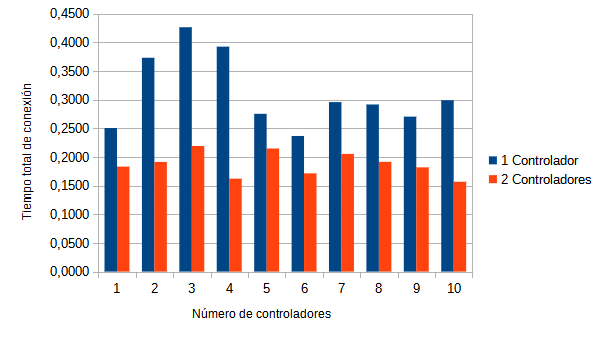
\includegraphics[width=13cm, keepaspectratio]{img/comparativaescenario4}
		\caption{Comparativa de tiempos en el cuarto escenario}
		\label{figura:comparativaescenario4}
	\end{figure}
	
	\begin{figure}[H]
		\centering
		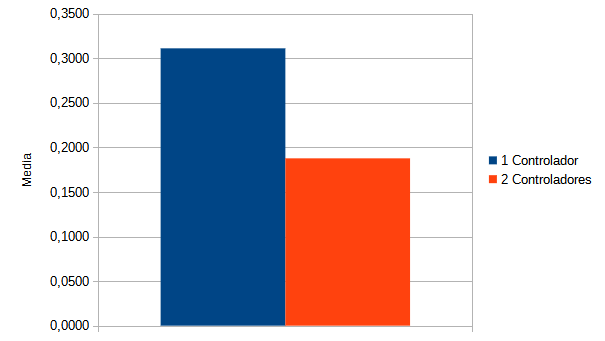
\includegraphics[width=13cm, keepaspectratio]{img/comparativamediaescenario4}
		\caption{Comparativa de media de tiempos en el cuarto escenario}
		\label{figura:mediaescenario4}
	\end{figure}
	

	
%	Además, hemos comprobado que por lo general el reparto de switches entre los controladores se ha realizado de forma correcta.

	
%%	\begin{figure}[H]
%		\centering
%		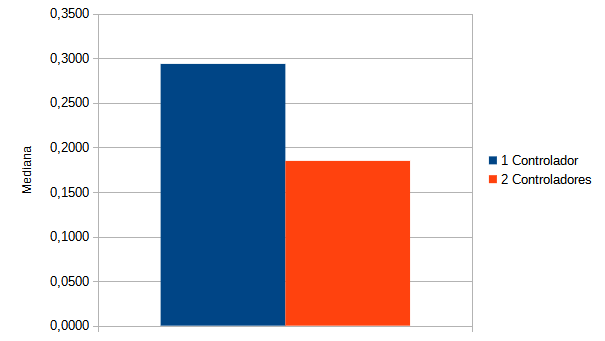
\includegraphics[width=12cm, keepaspectratio]{img/comparativamedianaescenario4}
%		\caption{Comparativa de medianas en el cuarto escenario}
%		\label{figura:medianae4}
%	\end{figure}
%	
%	\begin{figure}[H]
%		\centering
%		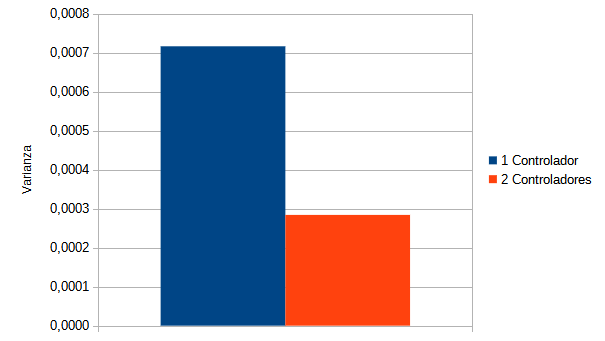
\includegraphics[width=12cm, keepaspectratio]{img/comparativavarianzaescenario4}
%		\caption{Comparativa de varianza de tiempos en el cuarto escenario}
%		\label{figura:varianzae4}
%	\end{figure}
		
	\begin{figure}[H]
		\centering
		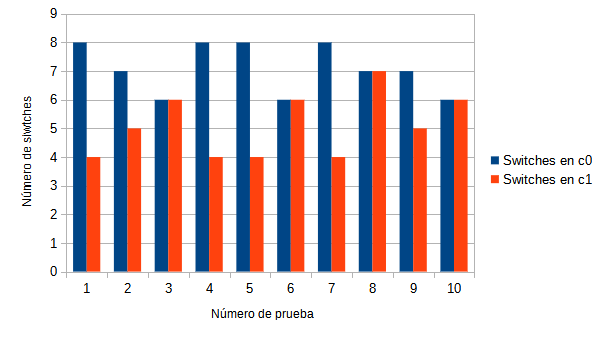
\includegraphics[width=16cm, keepaspectratio]{img/switchesporcontrollerescenario3}
		\caption{Número de switches por controlador.}
		\label{figura:switchesporcontrollerescenario4}
	\end{figure}
	

	
	Ahora veremos las comparativa también con el escenario con 4 controladores.
	
	\begin{figure}[H]
		\centering
		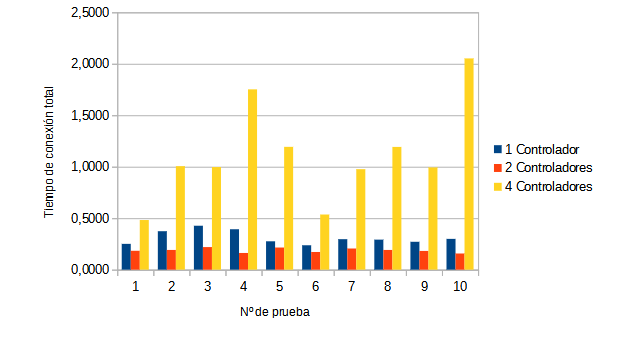
\includegraphics[width=16cm, keepaspectratio]{img/comparativaFail}
		\caption{Comparativa de tiempos en el cuarto escenario con los 3 experimentos}
		\label{figura:comparativaFail}
	\end{figure}
	
	En este gráfico, esta vez vemos que no ha habido mejora, sino que ha habido un empeoramiento muy  significativo. Puede ser debido a problemas con la máquina donde se realizaban los experimentos, o debido al propio experimento. Lo que en ambos casos puede significar que una sobrecarga de controladores, puede perjudicar el funcionamiento de este escenario.
	
	
	%%%%%%%%%%%%%%%%%%%%%%%%%%%%%%%%%%%%%%%%%%%%%%%%%%%%%%%%%%%%%%%%%%%%%%%%%%%%%%%%
	%%%%%%%%%%%%%%%%%%%%%%%%%%%%%%%%%%%%%%%%%%%%%%%%%%%%%%%%%%%%%%%%%%%%%%%%%%%%%%%%
	% CONCLUSIONES %
	%%%%%%%%%%%%%%%%%%%%%%%%%%%%%%%%%%%%%%%%%%%%%%%%%%%%%%%%%%%%%%%%%%%%%%%%%%%%%%%%
	
	\clearpage
	\chapter{Conclusiones}
	\label{chap:conclusiones}
	
	Como conclusión de lo visto en los diferentes experimentos, podemos confirmar que añadir un controlador a un escenario, va a ayudar a la hora de minimizar tiempos de conexión. Además, dicho tiempo mejorará cuanto mas lejos estén los nuevos controladores de los actuales del sistema, ya que los controladores tendrán que dar menos saltos, y por tanto, se reducirá el tiempo final. 
	
	\section{Consecución de objetivos}
	\label{sec:consecucion-objetivos}
	
	Como pudimos ver en el apartado ~\ref{chap:objetivos}, se pretendía conocer mejor el funcionamiento de OpenFlow con respecto al número de controladores, y en cada escenario hemos podido ver nuevas casuísticas que nos han ido aportando nueva información sobre el ya mencionado protocolo de comunicación. Con el primer escenario, que era el más pequeño y el que se puede estudiar más en profundidad, ya se pudo vislumbrar como iban a funcionar el resto de escenarios, que en efecto, han confirmado las hipótesis que planteamos con dichos resultados del escenario 1.
	
	Asimismo, con el ultimo experimento, hemos comprobado que no es siempre productivo añadir controladores, ya que una sobrecarga de éstos puede empeorar significativamente nuestros resultados.
	
	\section{Aplicación de lo aprendido}
	\label{sec:aplicacion}
	
	\begin{enumerate}
		\item Arquitectura de Redes de Ordenadores. Primer contacto con las redes de ordenadores, protocolos de comunicación, etc.
		\item Sistemas Telemáticos. Continuación de Arquitectura de Redes de Ordenadores, donde se profundizaba mas en materia.
	\end{enumerate}
	
	
	\section{Lecciones aprendidas}
	\label{sec:lecciones_aprendidas}
	
	A raíz de empezar a investigar para poder realizar el presente TFG hemos podido adquirir conocimientos en lo que respecta a:
	
	\begin{enumerate}
		\item OpenFlow. Al ser el elemento principal de esta investigación, la mayor parte de conocimiento que he adquirido ha sido sobre el protocolo de comunicación OpenFlow. El protocolo OpenFlow establece una comunicación entre el controlador y los dispositivos de red mediante mensajes definidos. El controlador puede enviar instrucciones a los dispositivos de red, como reglas de enrutamiento o de flujo, y recibir información sobre el estado de la red, como estadísticas de tráfico. Esto permite una gestión centralizada y programable de la red, lo que facilita la implementación de políticas de red, la optimización del tráfico y la resolución de problemas.
		\item LaTeX, ya que la memoria se ha realizado íntegramente con LaTeX. Con la ayuda de la plantilla hecha por el profesor Gregorio Robles y sus indicaciones, ha sido bastante sencillo realizar la documentación con dicha herramienta.
		\item Python. Pese a que el trabajo en si no tenía programación, he tenido que aprender las bases del lenguaje para entender los Scripts que se han utilizado tanto para definir los escenarios como para la realización de las pruebas.
		\item Desarrollar actitudes de investigación.
		
	\end{enumerate}
	
	
	\section{Trabajos futuros}
	\label{sec:trabajos_futuros}
	
	Tras realizar el presente TFG y visto lo aprendido y analizado el contenido del mismo, considero que sería una buena opción a tener en cuenta el optimizar los escenarios del sistema, creando lógica en los controladores, con el objetivo de evitar saturar determinados switches. Asimismo opino que podría ser interesante investigar sobre hasta que punto es factible añadir controladores extra a un escenario, ya que posiblemente llegue un punto que la mejora no sea lo suficientemente satisfactoria.
	
	
	%%%%%%%%%%%%%%%%%%%%%%%%%%%%%%%%%%%%%%%%%%%%%%%%%%%%%%%%%%%%%%%%%%%%%%%%%%%%%%%%
	%%%%%%%%%%%%%%%%%%%%%%%%%%%%%%%%%%%%%%%%%%%%%%%%%%%%%%%%%%%%%%%%%%%%%%%%%%%%%%%%
	% APÉNDICE(S) %
	%%%%%%%%%%%%%%%%%%%%%%%%%%%%%%%%%%%%%%%%%%%%%%%%%%%%%%%%%%%%%%%%%%%%%%%%%%%%%%%%
	
	\cleardoublepage
	
	%%%%%%%%%%%%%%%%%%%%%%%%%%%%%%%%%%%%%%%%%%%%%%%%%%%%%%%%%%%%%%%%%%%%%%%%%%%%%%%%
	%%%%%%%%%%%%%%%%%%%%%%%%%%%%%%%%%%%%%%%%%%%%%%%%%%%%%%%%%%%%%%%%%%%%%%%%%%%%%%%%
	% BIBLIOGRAFIA %
	%%%%%%%%%%%%%%%%%%%%%%%%%%%%%%%%%%%%%%%%%%%%%%%%%%%%%%%%%%%%%%%%%%%%%%%%%%%%%%%%
	
	\cleardoublepage
	
	% Las siguientes dos instrucciones es todo lo que necesitas
	% para incluir las citas en la memoria
	\bibliographystyle{abbrv}
	\bibliography{memoria} 
	
	[1]  A robust and reactive
	OpenFlow In-Band SDN Control Plane
	Version 0.1. Autores Pedro de las Heras y Eva María Castro. 2022
	
	[2]  Página informativa de OpenFlow https://noviflow.com/the-basics-of-sdn-and-the-openflow-network-architecture/ 
		
	[3]  Guía de LaTex.  https://github.com/gregoriorobles/plantilla-memoria/blob/master/memoria.tex
	
	[4]  Foundations of Modern Networking: SDN, NFV, QoE, IoT, and Cloud By William Stallings 2015
	
	[5]  Introducción a namespaces https://man7.org/linux/man-pages/man8/ip-netns.8.html
	
	[6]  Introducción a openvswitch http://openvswitch.org
	
	[7]  Introducción a Mininet http://mininet.org
	
	[8]  Continuación Mininet https://www.youtube.com/live/90fBCO1MMTA?si=uVvZdvl4D7t8ntFw
	
	[9]  Documentación de Networking http://docs.openstack.org
	
	[10] Documentación Linux Networking https://www.opencloudblog.com/
	
	[11] Documentación Faucet https://docs.faucet.nz/en/latest/tutorials/
 	
	 % memoria.bib es el nombre del fichero que contiene
	% las referencias bibliográficas. Abre ese fichero y mira el formato que tiene,
	% que se conoce como BibTeX. Hay muchos sitios que exportan referencias en
	% formato BibTeX. Prueba a buscar en http://scholar.google.com por referencias
	% y verás que lo puedes hacer de manera sencilla.
	% Más información: 
	% http://texblog.org/2014/04/22/using-google-scholar-to-download-bibtex-citations/
	
\end{document}
